%%%  کلاس AUTthesis، نسخه آبان 1397
%%%   دانشگاه صنعتی امیرکبیر                 http://www.aut.ac.ir
%%%  تالار گفتگوی پارسی‌لاتک،       http://forum.parsilatex.com
%%%   آپدیت شده در آبان 95
%%%   پشتیبانی و راهنمایی          badali_farhad@yahoo.com
%%%
%%%   بازبینی و اصلاح شده در آبان ماه 1397
%%%  Tested via TeXstudio in TeXlive 2014-2018.
%%%

%-----------------------------------------------------------------------------------------------------
%        روش اجرا.: 2 بار F1 ، 2 بار  F11(به منظور تولید مراجع) ، دوبار Ctrl+Alt+I (به منظور تولید نمایه) و دو بار F1 -------> مشاهده Pdf
%%%%%%%%%%%%%%%%%%%%%%%%%%%%%%%%%%%%%%%%%%%%%%%%%%%%%%
%   TeXstudio as your IDE
%%  برای compile در TeXstudio تنها کافی است منوی Options->Configure TeXstudio را زده و در پنجره Configure TeXstudio در بخش Build گزینه Default Compiler را به XeLaTeX تغییر دهید. سند شما به راحتی compile خواهد شد.
%   F1 & F5 : Build & view
%   F6      : Compile
%   F7      : View
%   --------------
%%%%%%%%%%%%%%%%%%%%%%%%%%%%%%%%%%%%%%%%%%%%%%%%%%%%%%
%        اگر قصد نوشتن رساله دکتری را دارید، در خط زیر به جای msc،
%      کلمه phd را قرار دهید. کلیه تنظیمات لازم، به طور خودکار، اعمال می‌شود.
%%% !TEX TS-program = XeLaTeX
\documentclass[oneside,msc,12pt]{AUTthesis}
%       فایل commands.tex را حتماً به دقت مطالعه کنید؛ چون دستورات مربوط به فراخوانی بسته زی‌پرشین 
%       و دیگر بسته‌ها و ... در این فایل قرار دارد و بهتر است که با نحوه استفاده از آنها آشنا شوید. توجه شود برای نسخه نهایی پایان‌نامه حتماً hyperref را 
%        غیرفعال کنید.


% در این فایل، دستورها و تنظیمات مورد نیاز، آورده شده است.
%-------------------------------------------------------------------------------------------------------------------
% در ورژن جدید زی‌پرشین برای تایپ متن‌های ریاضی، این سه بسته، حتماً باید فراخوانی شود.
\usepackage{amsthm,amssymb,amsmath,amsfonts}
% بسته‌ای برای تنطیم حاشیه‌های بالا، پایین، چپ و راست صفحه
\usepackage[top=30mm, bottom=30mm, left=25mm, right=30mm]{geometry}
% بسته‌‌ای برای ظاهر شدن شکل‌ها و تصاویر متن
\usepackage{graphicx}
%\usepackage{subfigure}
%\usepackage{subcaption}

\usepackage{color}
\usepackage[table]{xcolor}

%%%% Page color
\definecolor{cream}{rgb}{1.0, 0.99, 0.82}
\definecolor{floralwhite}{rgb}{1.0, 0.98, 0.94}
\definecolor{ghostwhite}{rgb}{0.97, 0.97, 1.0}
\definecolor{honeydew}{rgb}{0.94, 1.0, 0.94}
\definecolor{isabelline}{rgb}{0.96, 0.94, 0.93}
\definecolor{magnolia}{rgb}{0.97, 0.96, 1.0}
\definecolor{mintcream}{rgb}{0.96, 1.0, 0.98}
\definecolor{oldlace}{rgb}{0.99, 0.96, 0.9}
\definecolor{whitesmoke}{rgb}{0.96, 0.96, 0.96}
\definecolor{whitegray}{rgb}{0.98, 0.98, 0.98}
\definecolor{LightCyan}{rgb}{0.88,1,1}

\usepackage{listings}

\definecolor{dkgreen}{rgb}{0,0.6,0}
\definecolor{gray}{rgb}{0.5,0.5,0.5}
\definecolor{lightgray}{rgb}{0.8,0.8,0.8}
\definecolor{mauve}{rgb}{0.58,0,0.82}

\lstset{frame=tBLr,
%	frameround=fttt,
	language=python,
	aboveskip=3mm,
	belowskip=3mm,
	showstringspaces=false,
	columns=flexible,
	basicstyle={\small\ttfamily},
	lineskip=0.5em,
	xleftmargin=23pt,
	xrightmargin=9pt,
	framexleftmargin=17pt,
	framexrightmargin=5pt,
	framexbottommargin=2pt,
	numbers=left,
	firstnumber=1,
	numberstyle=\tiny\color{gray},
	keywordstyle=\color{blue},
	commentstyle=\color{dkgreen},
	stringstyle=\color{mauve},
	rulecolor=\color{black},
	breaklines=true,
	breakatwhitespace=true,
	tabsize=4
}
%\lstset{
%	language=python,
%	frame=trBL,  
%%	frameround=fttt,
%	numberstyle=\tiny\color{gray},
%	keywordstyle=\color{blue},
%	commentstyle=\color{dkgreen},
%	stringstyle=\color{mauve},
%	numbers=left,
%	numberstyle=\scriptsize,
%	showspaces=false,         
%	showtabs=false,       
%	xleftmargin=23pt,
%	xrightmargin=9pt,
%	framexleftmargin=17pt,
%	framexrightmargin=5pt,
%	framexbottommargin=2pt,
%	showstringspaces=false ,
%	breaklines=true,
%	texcl=true,
%	basicstyle=\setLTR\footnotesize\ttfamily,
%	lineskip=0.5em,
%	commentstyle= \itshape,
%	belowcaptionskip=12pt,
%	aboveskip=15pt,
%	belowskip=15pt
%}  
\newcommand{\code}[2][python]{
	\begin{latin}
%		\noindent #2
		\lstinputlisting[language=#1]{code/#2}
	\end{latin}
}
\definecolor{backgroundcode}{HTML}{FBFBFB}

\colorlet{punct}{red!60!black}
%\definecolor{background}{HTML}{EEEEEE}
\definecolor{delim}{RGB}{20,105,176}
\colorlet{numb}{magenta!60!black}
\definecolor{darkbrown}{rgb}{0.4, 0.26, 0.13}
\definecolor{darkblue}{rgb}{0.0, 0.0, 0.55}




\lstdefinelanguage{json}{
%	basicstyle=\normalfont\ttfamily,
	basicstyle=\scriptsize\ttfamily,
%	numbers=left,	
	numbers=none,
	numberstyle=\scriptsize,
	stepnumber=1,
	numbersep=8pt,
	showstringspaces=false,
	breaklines=true,
	breakatwhitespace=false,
	breakindent=0pt,
	frame=single,
	xleftmargin=10pt,
	xrightmargin=10pt,
	framexleftmargin=5pt,
	framexrightmargin=5pt,
		string=[s]{"}{"},
		comment=[l]{:\ "},
		morecomment=[l]{:"},
	moredelim=**[is][\color{red}]{@}{@},
	backgroundcolor=\color{backgroundcode},
	stringstyle=\color{black}, % style of strings
	literate=%
	*{0}{{{\color{numb}0}}}{1}
	{1}{{{\color{numb}1}}}{1}
	{2}{{{\color{numb}2}}}{1}
	{3}{{{\color{numb}3}}}{1}
	{4}{{{\color{numb}4}}}{1}
	{5}{{{\color{numb}5}}}{1}
	{6}{{{\color{numb}6}}}{1}
	{7}{{{\color{numb}7}}}{1}
	{8}{{{\color{numb}8}}}{1}
	{9}{{{\color{numb}9}}}{1}
	{e+}{{{\color{darkbrown}{e+}}}}{1}	
	{e-}{{{\color{darkbrown}{e-}}}}{1}
	{:}{{{\color{punct}{:}}}}{1}
	{,}{{{\color{punct}{,}}}}{1}
	{.}{{{\color{darkbrown}{.}}}}{1}
	{"}{{{\color{darkblue}{"}}}}{1}
	{'}{{{\color{red}{'}}}}{1}
   {\{}{{{\color{delim}\{}}}{1}
   {\}}{{{\color{delim}{\}}}}}{1}
	{[}{{{\color{delim}{[}}}}{1}
	{]}{{{\color{delim}{]}}}}{1},
}

%
%\definecolor{eclipseStrings}{RGB}{42,0.0,255}
%\definecolor{eclipseKeywords}{RGB}{127,0,85}
%\colorlet{numb}{magenta!60!black}
%
%\lstdefinelanguage{json}{
%	basicstyle=\normalfont\ttfamily,
%	commentstyle=\color{dkgreen}, % style of comment
%	stringstyle=\color{mauve}, % style of strings
%%	numbers=left,
%	numbers=none,
%	numberstyle=\scriptsize,
%	stepnumber=1,
%	numbersep=8pt,
%	showstringspaces=false,
%	breaklines=true,
%	frame=single,
%	backgroundcolor=\color{backgroundcode}, %only if you like
%	string=[s]{"}{"},
%	comment=[l]{:\ "},
%	morecomment=[l]{:"},
%	literate=
%	*{0}{{{\color{numb}0}}}{1}
%	{1}{{{\color{numb}1}}}{1}
%	{2}{{{\color{numb}2}}}{1}
%	{3}{{{\color{numb}3}}}{1}
%	{4}{{{\color{numb}4}}}{1}
%	{5}{{{\color{numb}5}}}{1}
%	{6}{{{\color{numb}6}}}{1}
%	{7}{{{\color{numb}7}}}{1}
%	{8}{{{\color{numb}8}}}{1}
%	{9}{{{\color{numb}9}}}{1}
%}
%




%بسته‌ای برای تنظیم فاصله عمودی خط‌های متن
\usepackage{setspace}
\usepackage{titletoc}
\usepackage{subfigure}
\usepackage[subfigure]{tocloft}
%\usepackage{tocloft}
%\setlength{\abovecaptionskip}{10pt plus 3pt minus 2pt} % Chosen fairly arbitrarily


\usepackage{array}%,makecell, cellspace}
%\newcommand{\tablewidth}{\def\arraystretch{5}}
\newcommand{\tableset}[2][2.0]{\centering\renewcommand{\arraystretch}{#1}{#2}}
\newcolumntype{C}[1]{>{\centering\arraybackslash}p{#1}}



\usepackage{tikz}
\newcommand*\circled[1]{\tikz[baseline=(char.base)]{\node[shape=circle,fill=blue!20,draw,inner sep=2pt] (char) {#1};}}

%با فعال کردن بسته زیر فوت‌نوت‌ها در هر صفحه ریست می‌شوند. حالت پیش‌فرض آن ریست شدن در هر فصل می‌باشد.
%\usepackage[perpage]{footmisc}
\usepackage[inline]{enumitem}
\newlist{alphinline}{enumerate*}{1}
\setlist[alphinline]{label=(\alph*)}
\newlist{enuminline}{enumerate*}{1}
\setlist[enuminline]{label=(\arabic*)}
\newlist{circlelist}{enumerate}{1}
\setlist[circlelist,1]{label=\protect\circled{\arabic*}}
\newlist{alphabetlist}{enumerate}{1}
\setlist[alphabetlist]{label=\alph*)}


%\usepackage{titlesec}
% بسته‌ و دستوراتی برای ایجاد لینک‌های رنگی با امکان جهش
\usepackage[pagebackref=false,colorlinks,linkcolor=blue,citecolor=red]{hyperref}
\usepackage[nameinlink]{cleveref}%capitalize,,noabbrev
 \AtBeginDocument{%
    \crefname{equation}{برابری}{equations}%
    \crefname{chapter}{فصل}{chapters}%
    \crefname{section}{بخش}{sections}%
    \crefname{appendix}{پیوست}{appendices}%
    \crefname{enumi}{مورد}{items}%
    \crefname{footnote}{زیرنویس}{footnotes}%
    \crefname{figure}{شکل}{figures}%
    \crefname{table}{جدول}{tables}%
    \crefname{theorem}{قضیه}{theorems}%
    \crefname{lemma}{لم}{lemmas}%
    \crefname{corollary}{نتیجه}{corollaries}%
    \crefname{proposition}{گزاره}{propositions}%
    \crefname{definition}{تعریف}{definitions}%
    \crefname{result}{نتیجه}{results}%
    \crefname{example}{مثال}{examples}%
    \crefname{remark}{نکته}{remarks}%
    \crefname{note}{یادداشت}{notes}%
}
% چنانچه قصد پرینت گرفتن نوشته خود را دارید، خط بالا را غیرفعال و  از دستور زیر استفاده کنید چون در صورت استفاده از دستور زیر‌‌، 
% لینک‌ها به رنگ سیاه ظاهر خواهند شد که برای پرینت گرفتن، مناسب‌تر است
%\usepackage[pagebackref=false]{hyperref}
% بسته‌ لازم برای تنظیم سربرگ‌ها
\usepackage{fancyhdr}
% بسته‌ای برای ظاهر شدن «مراجع»  در فهرست مطالب
\usepackage[nottoc]{tocbibind}
% دستورات مربوط به ایجاد نمایه
\usepackage{makeidx,multicol}
\setlength{\columnsep}{1.5cm}

%%%%%%%%%%%%%%%%%%%%%%%%%%
\usepackage{verbatim}
\makeindex
\usepackage{sectsty}

\usepackage[xindy,acronym,nonumberlist=true]{glossaries}



% فراخوانی بسته زی‌پرشین و تعریف قلم فارسی و انگلیسی
\usepackage{xepersian}%[extrafootnotefeatures]
\SepMark{-}
%حتماً از تک لایو 2014 استفاده کنید.
\settextfont[Scale=1.2]{B Nazanin}
\setlatintextfont{Times New Roman}
\renewcommand{\labelitemi}{$\bullet$}
%%%%%%%%%%%%%%%%%%%%%%%%%%
% چنانچه می‌خواهید اعداد در فرمول‌ها، انگلیسی باشد، خط زیر را غیرفعال کنید.
%در غیر اینصورت حتماً فونت PGaramond را نصب کنید.
\setdigitfont[Scale=1.1]{Yas}
%%%%%%%%%%%%%%%%%%%%%%%%%%
% تعریف قلم‌های فارسی اضافی برای استفاده در بعضی از قسمت‌های متن
\defpersianfont\nastaliq[Scale=2]{IranNastaliq}
\defpersianfont\chapternumber[Scale=3]{B Nazanin}
%\chapterfont{\centering}%
%%%%%%%%%%%%%%%%%%%%%%%%%%
% دستوری برای تغییر نام کلمه «اثبات» به «برهان»
\renewcommand\proofname{\textbf{برهان}}

% دستوری برای تغییر نام کلمه «کتاب‌نامه» به «منابع و مراجع«
\renewcommand{\bibname}{منابع و مراجع}


% Headings for every page of ToC, LoF and Lot
\setlength{\cftbeforetoctitleskip}{-1.2em}
\setlength{\cftbeforelottitleskip}{-1.2em}
\setlength{\cftbeforeloftitleskip}{-1.2em}
\setlength{\cftaftertoctitleskip}{-1em}
\setlength{\cftafterlottitleskip}{-1em}
\setlength{\cftafterloftitleskip}{-1em}
%%\makeatletter
%%%%\renewcommand{\l@chapter}{\@dottedtocline{1}{1em\bfseries}{1em}}
%%%%\renewcommand{\l@section}{\@dottedtocline{2}{2em}{2em}}
%%%%\renewcommand{\l@subsection}{\@dottedtocline{3}{3em}{3em}}
%%%%\renewcommand{\l@subsubsection}{\@dottedtocline{4}{4em}{4em}}
%%%%\makeatother


\newcommand\tocheading{\par عنوان\hfill صفحه \par}
\newcommand\lofheading{\hspace*{.5cm}\figurename\hfill صفحه \par}
\newcommand\lotheading{\hspace*{.5cm}\tablename\hfill صفحه \par}

\renewcommand{\cftchapleader}{\cftdotfill{\cftdotsep}}
\renewcommand{\cfttoctitlefont}{\hspace*{\fill}\LARGE\bfseries}%\Large
\renewcommand{\cftaftertoctitle}{\hspace*{\fill}}
\renewcommand{\cftlottitlefont}{\hspace*{\fill}\LARGE\bfseries}%\Large
\renewcommand{\cftafterlottitle}{\hspace*{\fill}}
\renewcommand{\cftloftitlefont}{\hspace*{\fill}\LARGE\bfseries}
\renewcommand{\cftafterloftitle}{\hspace*{\fill}}

%%%%%%%%%%%%%%%%%%%%%%%%%%
% تعریف و نحوه ظاهر شدن عنوان قضیه‌ها، تعریف‌ها، مثال‌ها و ...
%برای شماره گذاری سه تایی قضیه ها
\theoremstyle{definition}
\newtheorem{definition}{تعریف}[section]
\newtheorem{remark}[definition]{نکته}
\newtheorem{note}[definition]{یادداشت}
\newtheorem{example}[definition]{نمونه}
\newtheorem{question}[definition]{سوال}
\newtheorem{remember}[definition]{یاداوری}
\theoremstyle{theorem}
\newtheorem{theorem}[definition]{قضیه}
\newtheorem{lemma}[definition]{لم}
\newtheorem{proposition}[definition]{گزاره}
\newtheorem{corollary}[definition]{نتیجه}
%%%%%%%%%%%%%%%%%%%%%%%%
%%%%%%%%%%%%%%%%%%%
%%% برای شماره گذاری چهارتایی قضیه ها و ...
%%\newtheorem{definition1}[subsubsection]{تعریف}
%%\newtheorem{theorem1}[subsubsection]{قضیه}
%%\newtheorem{lemma1}[subsubsection]{لم}
%%\newtheorem{proposition1}[subsubsection]{گزاره}
%%\newtheorem{corollary1}[subsubsection]{نتیجه}
%%\newtheorem{remark1}[subsubsection]{نکته}
%%\newtheorem{example1}[subsubsection]{مثال}
%%\newtheorem{question1}[subsubsection]{سوال}

%%%%%%%%%%%%%%%%%%%%%%%%%%%%

% دستورهایی برای سفارشی کردن صفحات اول فصل‌ها
\makeatletter
\newcommand\mycustomraggedright{%
 \if@RTL\raggedleft%
 \else\raggedright%
 \fi}
\def\@makechapterhead#1{%
\thispagestyle{style1}
\vspace*{20\p@}%
{\parindent \z@ \mycustomraggedright
\ifnum \c@secnumdepth >\m@ne
\if@mainmatter

\bfseries{\Huge \@chapapp}\small\space {\chapternumber\thechapter}
\par\nobreak
\vskip 0\p@
\fi
\fi
\interlinepenalty\@M 
\Huge \bfseries #1\par\nobreak
\vskip 120\p@

}

%\thispagestyle{empty}
\newpage}
\bidi@patchcmd{\@makechapterhead}{\thechapter}{\tartibi{chapter}}{}{}
\bidi@patchcmd{\chaptermark}{\thechapter}{\tartibi{chapter}}{}{}
\makeatother

\pagestyle{fancy}
\renewcommand{\chaptermark}[1]{\markboth{\chaptername~\tartibi{chapter}: #1}{}}

\fancypagestyle{style1}{
\fancyhf{} 
\fancyfoot[c]{\thepage}
\fancyhead[R]{\leftmark}%
\renewcommand{\headrulewidth}{1.2pt}
}


\fancypagestyle{style2}{
\fancyhf{}
\fancyhead[R]{چکیده}
\fancyfoot[C]{\thepage{}}
\renewcommand{\headrulewidth}{1.2pt}
}

\fancypagestyle{style3}{%
  \fancyhf{}%
  \fancyhead[R]{فهرست نمادها}
  \fancyfoot[C]{\thepage}%
  \renewcommand{\headrulewidth}{1.2pt}%
}

\fancypagestyle{style4}{%
  \fancyhf{}%
  \fancyhead[R]{فهرست جداول}
  \fancyfoot[C]{\thepage}%
  \renewcommand{\headrulewidth}{1.2pt}%
}

\fancypagestyle{style5}{%
  \fancyhf{}%
  \fancyhead[R]{فهرست اشکال}
  \fancyfoot[C]{\thepage}%
  \renewcommand{\headrulewidth}{1.2pt}%
}

\fancypagestyle{style6}{%
  \fancyhf{}%
  \fancyhead[R]{فهرست مطالب}
  \fancyfoot[C]{\thepage}%
  \renewcommand{\headrulewidth}{1.2pt}%
}

\fancypagestyle{style7}{%
  \fancyhf{}%
  \fancyhead[R]{نمایه}
  \fancyfoot[C]{\thepage}%
  \renewcommand{\headrulewidth}{1.2pt}%
}

\fancypagestyle{style8}{%
  \fancyhf{}%
  \fancyhead[R]{منابع و مراجع}
  \fancyfoot[C]{\thepage}%
  \renewcommand{\headrulewidth}{1.2pt}%
}
\fancypagestyle{style9}{%
  \fancyhf{}%
  \fancyhead[R]{واژه‌نامه‌ی فارسی به انگلیسی}
  \fancyfoot[C]{\thepage}%
  \renewcommand{\headrulewidth}{1.2pt}%
}
%


%دستور حذف نام لیست تصاویر و لیست جداول از فهرست مطالب
\newcommand*{\BeginNoToc}{%
  \addtocontents{toc}{%
    \edef\protect\SavedTocDepth{\protect\the\protect\value{tocdepth}}%
  }%
  \addtocontents{toc}{%
    \protect\setcounter{tocdepth}{-10}%
  }%
}
\newcommand*{\EndNoToc}{%
  \addtocontents{toc}{%
    \protect\setcounter{tocdepth}{\protect\SavedTocDepth}%
  }%
}
\newcounter{savepage}
\renewcommand{\listfigurename}{فهرست اشکال}
\renewcommand{\listtablename}{فهرست جداول}
%\renewcommand\cftsecleader{\cftdotfill{\cftdotsep}}
%%%%%%%%%%%%%%%%%%%%%%%%%%%%%
%%%%%%%%%%%%%%%%%%%%%%%%%%%%




%%%%%% ============================================================================================================
%\usepackage[xindy,acronym,nonumberlist=true]{glossaries}
%
%\usepackage{xepersian}%[extrafootnotefeatures]
%%%%%% ============================================================================================================

%%% تنظیمات مربوط به بسته  glossaries
%%% تعریف استایل برای واژه نامه فارسی به انگلیسی، در این استایل واژه‌های فارسی در سمت راست و واژه‌های انگلیسی در سمت چپ خواهند آمد. از حالت گروه ‌بندی استفاده می‌کنیم، 
%%% یعنی واژه‌ها در گروه‌هایی به ترتیب حروف الفبا مرتب می‌شوند، مثلا:
%%% الف
%%% افتصاد ................................... Economy
%%% اشکال ........................................ Failure
%%% ش
%%% شبکه ...................................... Network
\newglossarystyle{myFaToEn}{%
	\renewenvironment{theglossary}{}{}
	\renewcommand*{\glsgroupskip}{\vskip 10mm}
	\renewcommand*{\glsgroupheading}[1]{\subsection*{\glsgetgrouptitle{##1}}}
	\renewcommand*{\glossentry}[2]{\noindent\glsentryname{##1}\dotfill\space \glsentrytext{##1}
		
	}
}

%% % تعریف استایل برای واژه نامه انگلیسی به فارسی، در این استایل واژه‌های فارسی در سمت راست و واژه‌های انگلیسی در سمت چپ خواهند آمد. از حالت گروه ‌بندی استفاده می‌کنیم، 
%% % یعنی واژه‌ها در گروه‌هایی به ترتیب حروف الفبا مرتب می‌شوند، مثلا:
%% % E
%%% Economy ............................... اقتصاد
%% % F
%% % Failure................................... اشکال
%% %N
%% % Network ................................. شبکه

\newglossarystyle{myEntoFa}{%
	%%% این دستور در حقیقت عملیات گروه‌بندی را انجام می‌دهد. بدین صورت که واژه‌ها در بخش‌های جداگانه گروه‌بندی می‌شوند، 
	%%% عنوان بخش همان نام حرفی است که هر واژه در آن گروه با آن شروع شده است. 
	\renewenvironment{theglossary}{}{}
	\renewcommand*{\glsgroupskip}{\vskip 10mm}
	\renewcommand*{\glsgroupheading}[1]{\begin{latin} \subsection*{\glsgetgrouptitle{##1}} \end{latin}}
	%%% در این دستور نحوه نمایش واژه‌ها می‌آید. در این جا واژه فارسی در سمت راست و واژه انگلیسی در سمت چپ قرار داده شده است، و بین آن با نقطه پر می‌شود. 
	\renewcommand*{\glossentry}[2]{\noindent\glsentrytext{##1}\dotfill\space \glsentryname{##1}
		
	}
}

%%% تعیین استایل برای فهرست اختصارات
\newglossarystyle{myAbbrlist}{%
	%%% این دستور در حقیقت عملیات گروه‌بندی را انجام می‌دهد. بدین صورت که اختصارات‌ در بخش‌های جداگانه گروه‌بندی می‌شوند، 
	%%% عنوان بخش همان نام حرفی است که هر اختصار در آن گروه با آن شروع شده است. 
	\renewenvironment{theglossary}{}{}
	\renewcommand*{\glsgroupskip}{\vskip 10mm}
	\renewcommand*{\glsgroupheading}[1]{\begin{latin} \subsection*{\glsgetgrouptitle{##1}} \end{latin}}
	%%% در این دستور نحوه نمایش اختصارات می‌آید. در این جا حالت کوچک اختصار در سمت چپ و حالت بزرگ در سمت راست قرار داده شده است، و بین آن با نقطه پر می‌شود. 
	\renewcommand*{\glossentry}[2]{\noindent\glsentrytext{##1}\dotfill\space \Glsentrylong{##1}
		
	}
	%%% تغییر نام محیط abbreviation به فهرست اختصارات
	\renewcommand*{\acronymname}{\rl{فهرست اختصارات}}
}

%%% برای اجرا xindy بر روی فایل .tex و تولید واژه‌نامه‌ها و فهرست اختصارات و فهرست نمادها یکسری  فایل تعریف شده است.‌ Latex داده های مربوط به واژه نامه و .. را در این 
%%%  فایل‌ها نگهداری می‌کند. مهم‌ترین option‌ این قسمت این است که 
%%% عنوان واژه‌نامه‌ها و یا فهرست اختصارات و یا فهرست نمادها را می‌توانید در این‌جا مشخص کنید. 
%%% در این جا عباراتی مثل glg، gls، glo و ... پسوند فایل‌هایی است که برای xindy بکار می‌روند. 
\newglossary[glg]{english}{gls}{glo}{واژه‌نامه انگلیسی به فارسی}
\newglossary[blg]{persian}{bls}{blo}{واژه‌نامه فارسی به انگلیسی}
\makeglossaries
\glsdisablehyper
%%% تعاریف مربوط به تولید واژه نامه و فهرست اختصارات و فهرست نمادها
%%%  در این فایل یکسری دستورات عمومی برای وارد کردن واژه‌نامه آمده است.
%%%  به دلیل این‌که قرار است این دستورات پایه‌ای را بازنویسی کنیم در این‌جا تعریف می‌کنیم. 
\let\oldgls\gls
\let\oldglspl\glspl

\makeatletter

\renewrobustcmd*{\gls}{\@ifstar\@msgls\@mgls}
\newcommand*{\@mgls}[1] {\ifthenelse{\equal{\glsentrytype{#1}}{english}}{\oldgls{#1}\glsuseri{f-#1}}{\lr{\oldgls{#1}}}}
\newcommand*{\@msgls}[1]{\ifthenelse{\equal{\glsentrytype{#1}}{english}}{\glstext{#1}\glsuseri{f-#1}}{\lr{\glsentryname{#1}}}}

\renewrobustcmd*{\glspl}{\@ifstar\@msglspl\@mglspl}
\newcommand*{\@mglspl}[1] {\ifthenelse{\equal{\glsentrytype{#1}}{english}}{\oldglspl{#1}\glsuseri{f-#1}}{\oldglspl{#1}}}
\newcommand*{\@msglspl}[1]{\ifthenelse{\equal{\glsentrytype{#1}}{english}}{\glsplural{#1}\glsuseri{f-#1}}{\glsentryplural{#1}}}

\makeatother

\newcommand{\newword}[4]{
	\newglossaryentry{#1}     {type={english},name={\lr{#2}},plural={#4},text={#3},description={}}
	\newglossaryentry{f-#1} {type={persian},name={#3},text={\lr{#2}},description={}}
}

%%% بر طبق این دستور، در اولین باری که واژه مورد نظر از واژه‌نامه وارد شود، پاورقی زده می‌شود. 
\defglsentryfmt[english]{\glsgenentryfmt\ifglsused{\glslabel}{}{\LTRfootnote{\glsentryname{\glslabel}}}}

%%% بر طبق این دستور، در اولین باری که واژه مورد نظر از فهرست اختصارات وارد شود، پاورقی زده می‌شود. 
\defglsentryfmt[acronym]{\glsentryname{\glslabel}\ifglsused{\glslabel}{}{\LTRfootnote{\glsentrydesc{\glslabel}}}}


%%%%%% ============================================================================================================

%%============================ دستور برای قرار دادن فهرست اختصارات 
\newcommand{\printabbreviation}{
	\cleardoublepage
	\phantomsection
	\baselineskip=.75cm
	%% با این دستور عنوان فهرست اختصارات به فهرست مطالب اضافه می‌شود. 
	\addcontentsline{toc}{chapter}{فهرست اختصارات}
	\setglossarystyle{myAbbrlist}
	\begin{latin}
		\Oldprintglossary[type=acronym]	
	\end{latin}
	\clearpage
}%

\newcommand{\printacronyms}{\printabbreviation}
%%% در این جا محیط هر دو واژه نامه را باز تعریف کرده ایم، تا اولا مشکل قرار دادن صفحه اضافی را حل کنیم، ثانیا عنوان واژه نامه ها را با دستور addcontentlist وارد فهرست مطالب کرده ایم.
\let\Oldprintglossary\printglossary
\renewcommand{\printglossary}{
	\let\appendix\relax
	%% تنظیم کننده فاصله بین خطوط در این قسمت
	\clearpage
	\phantomsection
	%% این دستور موجب این می‌شود که واژه‌نامه‌ها در  حالت دو ستونی نوشته شود. 
	\twocolumn{}
	%% با این دستور عنوان واژه‌نامه به فهرست مطالب اضافه می‌شود. 
	\addcontentsline{toc}{chapter}{واژه نامه انگلیسی به فارسی}
	\setglossarystyle{myEntoFa}
	\Oldprintglossary[type=english]
	
	\clearpage
	\phantomsection
	%% با این دستور عنوان واژه‌نامه به فهرست مطالب اضافه می‌شود. 
	\addcontentsline{toc}{chapter}{واژه نامه فارسی به انگلیسی}
	\setglossarystyle{myFaToEn}
	\Oldprintglossary[type=persian]
	\onecolumn{}
}%

% ===============================================================================================================


%xindy -L persian-variant1 -C utf8 -I xindy -M %.xdy -t %.glg -o %.gls %.glo | 
%xindy -L persian-variant1 -C utf8 -I xindy -M %.xdy -t %.blg -o %.bls %.blo |
%xindy -L english -C utf8 -I xindy -M %.xdy -t %.alg -o %.acr %.acn


%xindy -M texindy -C utf8 -L persian-varient2 %.idx

%!main=AUTthesis
%===============
%%% نحوه تعریف واژگان 

\newword{RandomVariable}{Random Variable}
{متغیر تصادفی}{متغیرهای تصادفی}

\newword{w:action}{Action}{حرکت}{حرکت}
\newword{w:state}{State}{حرکت}{حرکت}
\newword{w:reward}{Reward}{امتیاز}{امتیاز}
\newword{w:env}{Environment}{محیط}{محیط}
\newword{w:agent}{Agent}{عامل}{عامل}

\newword{w:actionspace}{Action Space}{فضای حرکت}{فضای حرکت}
\newword{w:obsspace}{Observation Space}{فضای مشاهده}{فضای مشاهده}

\newword{w:matlab}{Matlab}{نرم‌افزار متلب}{متلب}
\newword{w:simulink}{Simulink}{سیمولینک}{سیمولینک}
\newword{w:matlabengine}{Matlab Engine}{موتور متلب}{موتور متلب}
\newword{w:anaconda}{Anaconda}{نرم‌افزار آناکوندا}{آناکوندا}
\newword{w:prescan}{PreScan}{نرم‌افزار پری‌اسکن}{پری‌اسکن}
\newword{w:timeout}{Timeout}{سقف زمانی}{سقف زمانی}
\newword{w:episode}{Episode}{اپیزود}{اپیزود}
\newword{w:dyndata}{Dynamic Data}{داده‌های پویا}{داده‌های پویا}
\newword{w:drl}{Deep Reinforcement Learning}{یادگیری تقویتی عمیق}{یادگیری تقویتی عمیق}
\newword{w:ml}{Machine Learning}{یادگیری ماشین}{یادگیری ماشین}
%\newword{w:}{}{}{}
%\newword{w:}{}{}{}
%\newword{w:}{}{}{}
%\newword{w:}{}{}{}
%\newword{w:}{}{}{}
%\newword{w:}{}{}{}
%\newword{w:}{}{}{}
%\newword{w:}{}{}{}
%\newword{w:}{}{}{}
%\newword{w:}{}{}{}
%\newword{w:}{}{}{}
%\newword{w:}{}{}{}
%\newword{w:}{}{}{}




%%%%%% ============================================================================================================

%%% نحوه تعریف اختصارات
%\newacronym{DFT}{DFT}{Discrete Fourier Transform}
%\newacronym{CDMA}{CDMA}{Code Division Multiplexing Access}
%\newacronym{BAN}{BAN}{Body Area Network}



%%%%%% ============================================================================================================


\newcommand{\w}[1]{\glspl{w:#1}}
\newcommand{\ws}[1]{\glspl*{w:#1}}

%%%%%% ============================================================================================================


\begin{document}
\baselineskip=.75cm
\linespread{1.75}
%% -!TEX root = AUTthesis.tex
% در این فایل، عنوان پایان‌نامه، مشخصات خود، متن تقدیمی‌، ستایش، سپاس‌گزاری و چکیده پایان‌نامه را به فارسی، وارد کنید.
% توجه داشته باشید که جدول حاوی مشخصات پروژه/پایان‌نامه/رساله و همچنین، مشخصات داخل آن، به طور خودکار، درج می‌شود.
%%%%%%%%%%%%%%%%%%%%%%%%%%%%%%%%%%%%
% دانشکده، آموزشکده و یا پژوهشکده  خود را وارد کنید
\faculty{دانشکده مهندسی برق}
% گرایش و گروه آموزشی خود را وارد کنید
\department{گرایش مخابرات}
% عنوان پایان‌نامه را وارد کنید
\fatitle{ماشین های خودران- 
	\\[0.75cm]
	با استفاده از یادگیری تقویتی}
% نام استاد(ان) راهنما را وارد کنید
\firstsupervisor{دکتر وحید پوراحمدی}
\secondsupervisor{دکتر حمیدرضا امین‌داور}
% نام استاد(دان) مشاور را وارد کنید. چنانچه استاد مشاور ندارید، دستور پایین را غیرفعال کنید.
%\firstadvisor{دکتر عبدالعلی عبدی‌پور}
%\secondadvisor{استاد مشاور دوم}
% نام نویسنده را وارد کنید
\name{محمد }
% نام خانوادگی نویسنده را وارد کنید
\surname{رضیئی فیجانی}
%%%%%%%%%%%%%%%%%%%%%%%%%%%%%%%%%%
\thesisdate{شهریور ۱۳۹۸}

% چکیده پایان‌نامه را وارد کنید
\fa-abstract{
در اين قسمت چكيده پایان نامه نوشته مي‌شو‌د‌.‌ چكيده بايد جامع و بيان‌كننده‌ خلاصه‌اي از اقدامات انجام‌شده باشد. در چكيده باید از ارجاع به مرجع و ذكر روابط رياضي، بيان تاريخچه و تعريف مسئله خودداري ‌شود. 
}


% کلمات کلیدی پایان‌نامه را وارد کنید
\keywords{کلیدواژه اول، ...، کلیدواژه پنجم (نوشتن سه تا پنج واژه کلیدی ضروری است)}



\AUTtitle
%%%%%%%%%%%%%%%%%%%%%%%%%%%%%%%%%%
\vspace*{7cm}
\thispagestyle{empty}
\begin{center}

\includegraphics[height=5cm,width=12cm]{besm}
\end{center}
% تاییدیه دفاع
\newpage
\thispagestyle{empty}
%\fontsize{18pt}{19pt}\selectfont

\section*{صفحه فرم ارزیابی و تصویب پایان نامه- فرم تأیید اعضاء كميته دفاع}

\fontsize{12pt}{14pt}\selectfont
%\renewcommand{\baselinestretch}{1.5}
%\vspace*{1cm}
\begin{figure}[h!]
	\centering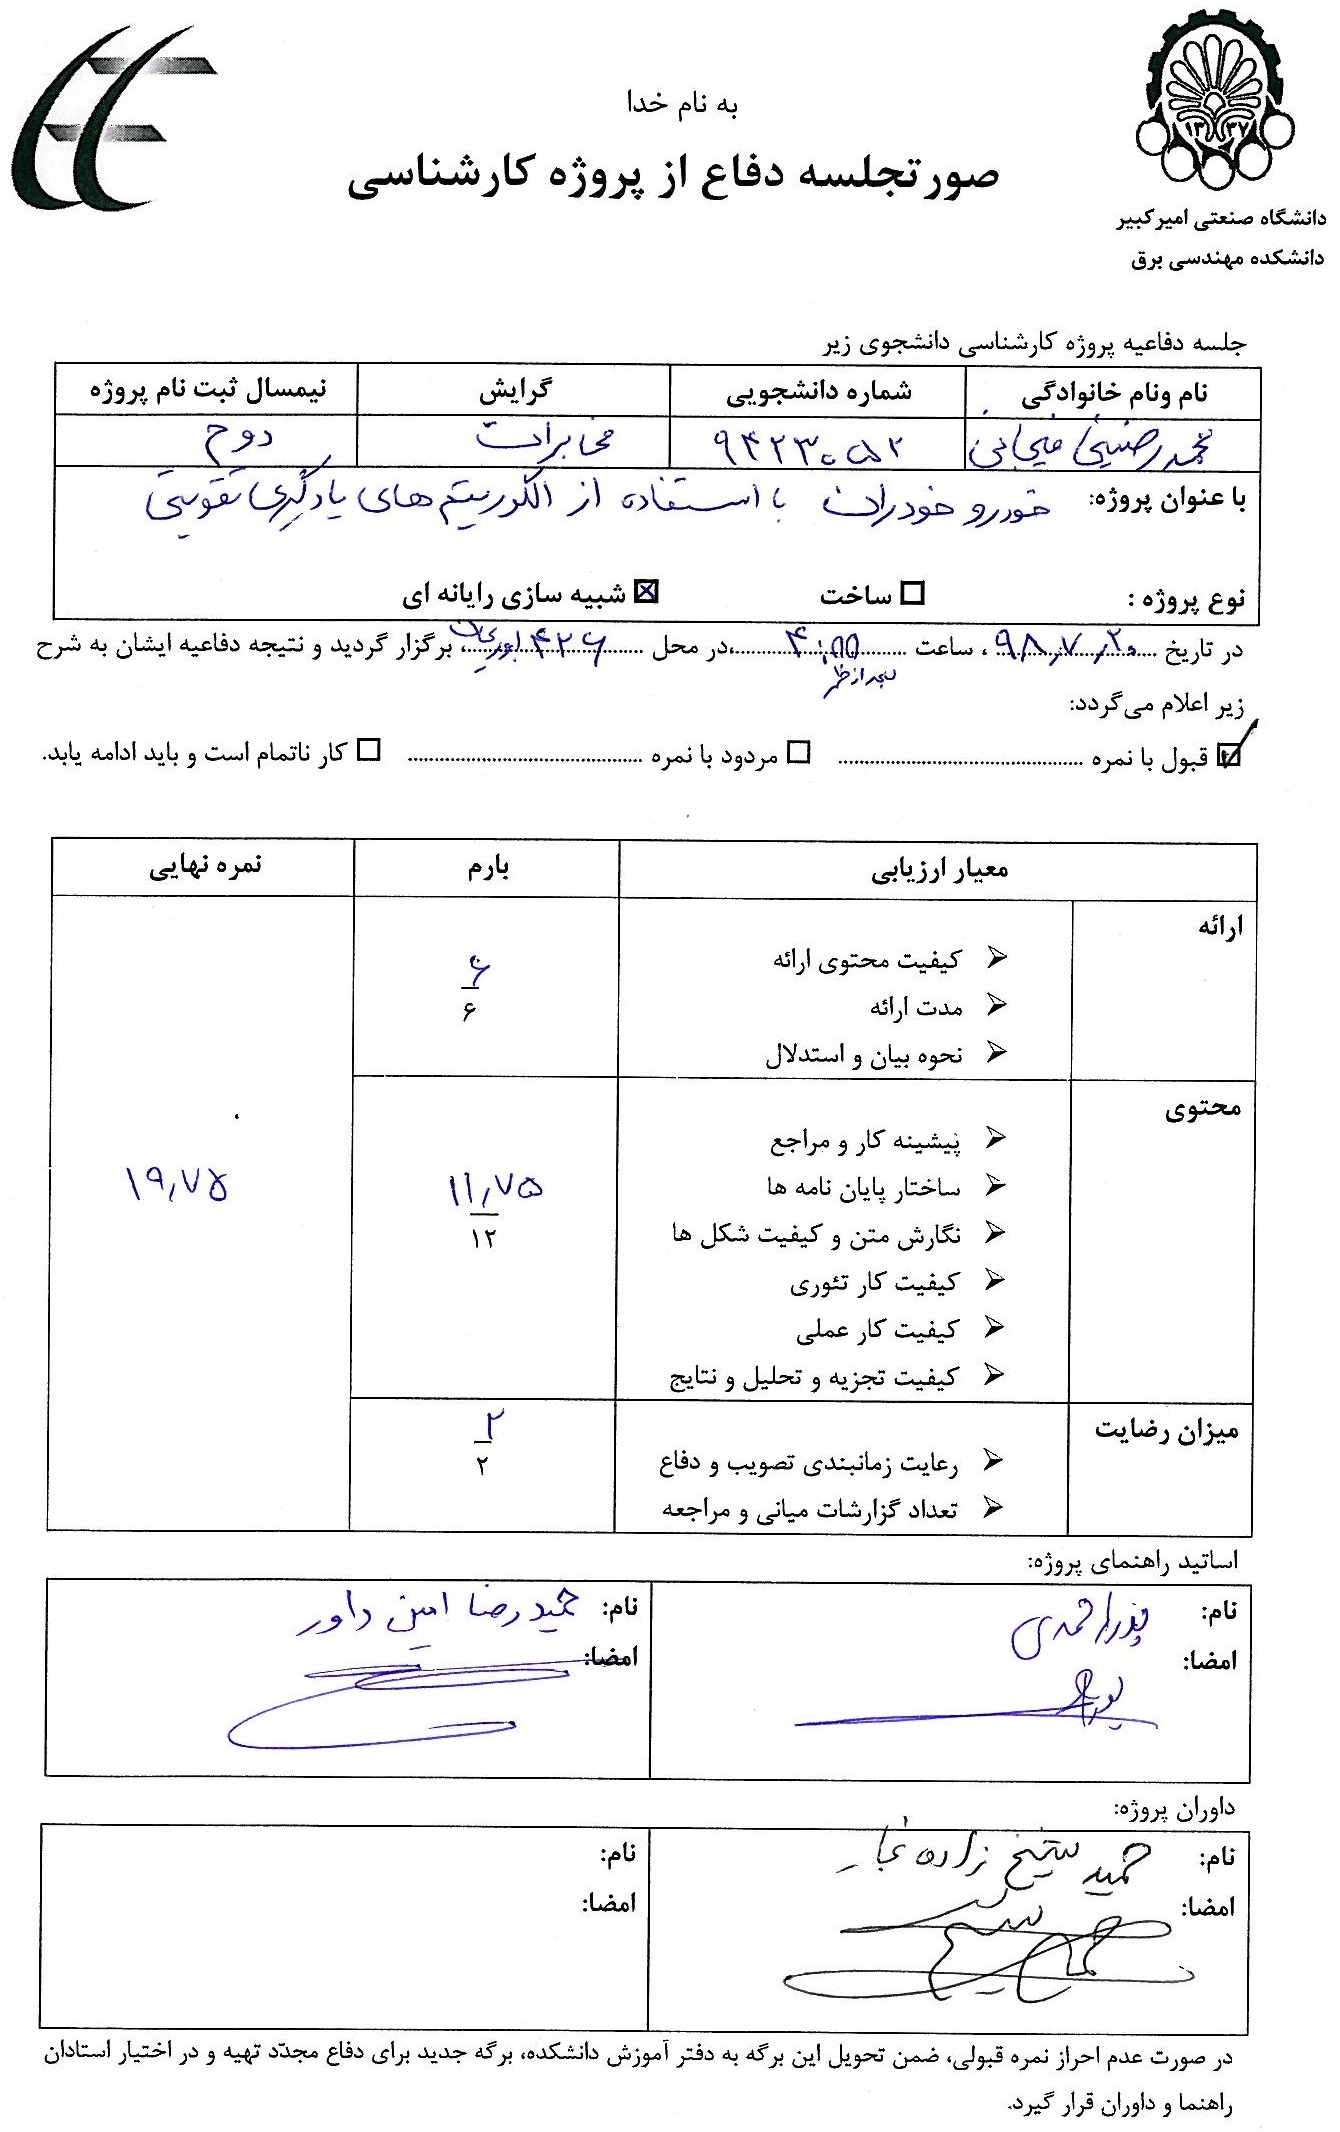
\includegraphics[width=0.82\linewidth]{tasvib2}
\end{figure}
%   در این صفحه فرم دفاع یا تایید و تصویب پایان نامه موسوم به فرم کمیته دفاع- موجود در پرونده آموزشی- را قرار دهید.
%\vspace*{1cm}
%
%
%\subsection*{نکات مهم:}
% 
%\begin{itemize}
%\item
%	نگارش پایان نامه/رساله باید به
%	{\color{red}
%		زبان فارسی
%	}
%	و بر اساس آخرین نسخه دستورالعمل و راهنمای تدوین پایان نامه های دانشگاه صنعتی امیرکبیر باشد.(دستورالعمل و راهنمای حاضر)
%\item رنگ جلد پایان نامه/رساله چاپي كارشناسي، كارشناسي ارشد و دكترا  بايد به ترتيب مشكي، طوسي و سفيد رنگ باشد.  
%\item چاپ و صحافی پایان نامه/رساله بصورت
%{\color{red}
%	پشت و رو(دورو)
%}
%بلامانع است و انجام آن توصيه مي شود. 
%\end{itemize}
%%%%%%%%%%%%%%%%%%%%%%%%%%%%%%%%%%%%%%%%%%%%%%%%%%%%%%%%%%%%%%%%%%%%%%%%%%%%%%%%%%%%%%%%%%%%%%%%%%
%%%%%%%%%%%%%%%%%%%%%%%%%%%%%%%%%%%%%%%%%%%%%%%%%%%%%%%%%%%%%%%%%%%%%%%%%%%%%%%%%%%%%%%%%%%%%%%%%%
\newpage
\thispagestyle{empty}
\begin{picture}(50,50)
  \put(17,0){
\includegraphics[scale=1.1]{fa-logo}}
  \put(4.5,-13){\footnotesize{دانشگاه صنعتی امیرکبیر}}
  \put(10.5,-27){\footnotesize{(پلی‌تکنیک تهران)}}
  \put(170,30){\bf{به نام خدا}}
  \put(140,-5){\Large\bf{تعهدنامه اصالت اثر}}
  \put(310,0){تاریخ: \datethesis}
\end{picture}

\vspace*{2.5cm}

اينجانب {\bf{\fname\lname}} متعهد می‌شوم که مطالب مندرج در این پایان‌نامه حاصل کار پژوهشی اینجانب تحت نظارت و راهنمایی اساتید دانشگاه صنعتی امیرکبیر بوده و به دستاوردهای دیگران که در این پژوهش از آنها استفاده شده است مطابق مقررات و روال متعارف ارجاع و در فهرست منابع و مآخذ ذکر گردیده است. این پایان‌نامه قبلاً برای احراز هیچ مدرک هم‌سطح یا بالاتر ارائه نگردیده است.

در صورت اثبات تخلف در هر زمان، مدرک تحصیلی صادر شده توسط دانشگاه از درجه اعتبار ساقط بوده و دانشگاه حق پیگیری قانونی خواهد داشت.


کلیه نتایج و حقوق حاصل از این پایان‌نامه متعلق به دانشگاه صنعتی امیرکبیر می‌باشد. هرگونه استفاده از نتایج علمی و عملی، واگذاری اطلاعات به دیگران یا چاپ و تکثیر، نسخه‌برداری، ترجمه و اقتباس از این پایان نامه بدون موافقت کتبی دانشگاه صنعتی امیرکبیر ممنوع است. 
نقل مطالب با ذکر مآخذ بلامانع است.\\
\vspace{2.5cm}


{\centerline {\bf{\fname\lname}}}
\vspace*{.2cm}
{\centerline{امضا}}
%%%%%%%%%%%%%%%%%%%%%%%%%%%%%%%%%
% چنانچه مایل به چاپ صفحات «تقدیم»، «نیایش» و «سپاس‌گزاری» در خروجی نیستید، خط‌های زیر را با گذاشتن ٪  در ابتدای آنها غیرفعال کنید.
% پایان‌نامه خود را تقدیم کنید
% نیایش خود را در فایل زیر بنویسید.
\begin{acknowledgementpage}

\vspace{1.5cm}

{\nastaliq
{
این پایان نامه را به پدر، مادر و برادرم که کمک کردند تا این پروژه به اتمام برسد تقدیم می‌کنم. 
همچنین امیدوارم این پروژه گامی نخست برای گام‌های فرا تر باشد.



}}\end{acknowledgementpage}
\newpage
% سپاسگزاری را در فایل زیر بنویسید.
%%%%%%%%%%%%%%%%%%%%%%%%%%%%%%%%%%%%
\newpage\thispagestyle{empty}
% سپاس‌گزاری
{\nastaliq
سپاس‌گزاری
}
\\[2cm]

از دکتر پوراحمدی و دکتر امین داور که کمک های فراوانی جهت پیش‌برد این هدف بزرگ داشته‌اند، کمال تشکر را دارم. همچنین از سایر دوستانی که من را در این پروژه همراهی و یاری دادند، بسیار متشکر هستم.













% با استفاده از دستور زیر، امضای شما، به طور خودکار، درج می‌شود.
\signature








%%%%%%%%%%%%%%%%%%%%%%%%%%%%%%%%%%%%%%%%%
%%%%%%%%%%%%%%%%%%%%%%%%%%%%%%%%%کدهای زیر را تغییر ندهید.
\newpage\clearpage

\pagestyle{style2}

\vspace*{-1cm}
\section*{\centering چکیده}
%\addcontentsline{toc}{chapter}{چکیده}
\vspace*{.5cm}
\ffa-abstract
\vspace*{2cm}


{\noindent\large\textbf{واژه‌های کلیدی:}}\par
\vspace*{.5cm}
\fkeywords
% دستور زیر برای شماره گذاری صفحات قبل از فصل اول با حروف ابجد است.
\pagenumbering{alph}
%-----------------------------------------------------------------------------
% فایل زیر دستورات مربوط به نمایش صفحات فهرست مطالب- فهرست اشکال و جداول است.
%{\pagestyle{style2}
%\tableofcontents}\newpage
%
%\listoffigures
\cleardoublepage
\pagestyle{style6}
\tableofcontents
\pagestyle{style6}
\cleardoublepage
%اگر لیست تصاویر و لیست جداول ندارید ، کدهای زیر را با گذاشتن % در ابتدای آنها، غیرفعال کنید.
\BeginNoToc
%============
\addtocontents{lof}{\lofheading}% add heading to the first page in LoF
\pagestyle{style5}
\listoffigures
\thispagestyle{style5}
\cleardoublepage
%============
\addtocontents{lot}{\lotheading}% add heading to the first page in LoT
\thispagestyle{style4}
\listoftables
\thispagestyle{style4}
%============
%\cleardoublepage
%
\cleardoublepage
\setcounter{savepage}{\arabic{page}}
\mainmatter
\addtocontents{toc}{\tocheading}% add heading to the first page in ToC, after frontmatter entries
\EndNoToc
% در صورت تمایل می‌توانید با فعال کردن دستور بالا، لیست تصاویر را به  پایان‌نامه خود اضافه کنید.
%-------------------------------------------------------------------------symbols(فهرست نمادها)
% وجود لیست نمادها الزامیست.(لطفاً نمادهای خود را جایگذین نمادهای پیش‌فرض کنید.)
%%%%%%%%%%%%%

{\centering\LARGE\textbf{فهرست نمادها}\par}%

\pagenumbering{alph}
\setcounter{page}{\thesavepage}
%\setcounter{page}{6}
\vspace*{1cm}

\pagestyle{style3}
%\thispagestyle{empty}
%\addcontentsline{toc}{chapter}{فهرست نمادها}
\symb{\text{ نماد}}{مفهوم}
\\
%مقادیر بالا را تغییر ندهید
%%%%%%%%%%%%%%%%%%%%%%%%%%%%%%%%%%%%%%%%%%%%%%%%%%%%%%%%%
\symb{\mathcal{R}_t}{
امتیاز آنی در لحظه $t$
}
\symb{\mathcal{S}_t}{
حالت در لحظه $t$
}
\symb{\mathcal{S}^a_t}{
	حالت عامل در لحظه $t$
}
\symb{\mathcal{S}^e_t}{
	حالت محیط در لحظه $t$
}
\symb{\mathcal{O}_t}{
مشاهده در لحظه $t$
}
\symb{\mathcal{A}_t}{
حرکت در لحظه $t$
}
\symb{\|\mathcal{O}\|}{
اندازه فضای مشاهده
}
\symb{\|\mathcal{A}\|}{
اندازه فضای حرکت
}
\symb{\mathcal{H}_t}{
تاریخچه تا لحظه $t$
}
\symb{\mathcal{G}_t}{
تابع تجمعی امتیاز، تابع بازگشت
}
\symb{\gamma}{
ضریب کاهنده
}
\symb{\left.F^{\mathcal{C}}\right|_a}{
تابع مرتبط با مفهوم $\mathcal{C}$ با پارامتر $a$
}
%
%\symb{L}{
%مشتق لی
%}
%\symb{\Phi}{
%2-فرم اساسی خمینه تماسی
%}
%\symb{\nabla}{
%التصاق لوی-چویتای
%}
%\symb{\Delta}{
%لاپلاسین ناهموار
%}
%\symb{\nabla^*}{
%عملگر خودالحاق صوری القا شده از التصاق لوی-چویتای
%}
%\symb{g_s}{
%متر ساساکی
%}
%\symb{\nabla}{
%التصاق لوی-چویتای وابسته به متر ساساکی
%}
%\symb{\Delta}{
%عملگر لاپلاس-بلترامی روی $p$-فرم‌ها
%}
%%%%%%%%%%%%%%%%%%%%%%%%%%%%%%%%%%%%%%%

\thispagestyle{style3}
\newpage
%\pagestyle{style1}
%%%%%%%%%%%%%%%%%%%%%%%%%%%%%%%%%%%%


\pagenumbering{arabic}
\pagestyle{style1}
%--------------------------------------------------------------------------chapters(فصل ها)
\chapter{مقدمه}

یادگیری تقویتی یکی از گرایش‌های یادگیری ماشینی است که از روانشناسی رفتاری الهام می‌گیرد. این روش بر رفتارهایی تمرکز دارد که ماشین باید برای بیشینه کردن پاداشش انجام دهد. این مسئله، با توجه به گستردگی‌اش، در زمینه‌های گوناگونی بررسی می‌شود. مانند: 
\begin{alphinline}
	\item
	نظریه بازی‌ها،
	\item  
	نظریه کنترل، 
	\item 
	تحقیق در عملیات،
	 \item 
	نظریه اطلاعات، 
	\item 
	سامانه چندعامله، 
	\item 
	هوش ازدحامی، 
	\item 
	آمار، 
	\item 
	الگوریتم ژنتیک، 
	\item
	بهینه‌سازی بر مبنای شبیه‌سازی. 
	
\end{alphinline}

حوزه خودران سازی خودرو ها در سال های اخیر طرفداران زیادی پیدا کرده است. شرکت های بسیاری در دنیا مانند تسلا، رولزرویس، دیپ مایند، گوگل و اخیرا اپل، در حوزه حمایت‌های زیادی از این گونه فعالیت ها داشته اند. الگوریتم های یادگیری تقویتی از آن جهت در این بین محبوب است که یک ماشین سعی می‌کند مانند یک کودک، فعالیت کند و تجربه کسب کند و بیاموزد و حرکت کند. در واقع، قوانین به صورت امتیاز و یا پاداش به این سیستم وارد می‌شوند بدون آن که به ناظر نیاز شود.

این الگوریتم ها در دسته سوم شاخه های یادگیری ماشین، یعنی یادگیری تقویتی در کنار دو شاخه دیگر یعنی یادگیری با ناظر و یادگیری بدون ناظر مطرح می‌شوند. بر خلاف بخش های دیگر این بخش ریاضیات قوی و کامل تری را شامل می‌شود. فرضیه ای در این حوزه به نام فرضیه امتیاز ها مطرح است که می‌گوید «همه اهداف را می‌توان با بیشینه کردن امید امتیاز های تجمعی توصیف کرد.»

در این پروژه سعی شد با استفاده از تعریف مناسب «مشاهده» و «امتیاز» ها و همچنین تعیین دیگر پارامتر های الگوریتم، به خودروی مورد مطالعه یاد بدهد که خودران شود. سرانجام این خودرو به صورت شبیه سازی شده شروع به حرکت کرد و مسیر را یاد گرفت.

به صورت کلی، این پروژه دو لایه کلی دارد؛ لایه الگوریتم و لایه شبیه ساز. 
لایه الگوریتم با استفاده از پایتون نوشته شده است اما لایه شبیه ساز با بکار گیری نرم افزار پری‌اسکن در محیط سیمولینک متلب این عمل صورت گرفته است. شایان ذکر است که دو لایه مذکور توسط نویسنده همین پایان‌نامه توسعه یافته‌اند. در حقیقت نوشتن یک محیط شبیه سازی (با قابلیت توسعه ساده در آینده)
از دستاورد های مهم و بخش اصلی این پروژه می‌باشد.


%
%همان‌طور که گفته شد، در این پروژه از ابزار های مختلفی استفاده شده است. همچنین از برخی ابزار دیگر نیز جهت ایجاد اتصال بین آن ابزار ها استفاده شده اند. در این بخش، این اجزا به تفصیل بررسی خواهد شد.
%
%هر کدام از این اجزا کار مشخصی را بر عهده دارند.
%شکل  
%\ref{fig:block-diagram2}
%این ارتباط را نشان می‌دهد.
%
%\begin{figure}[h!]
%	\centering
%	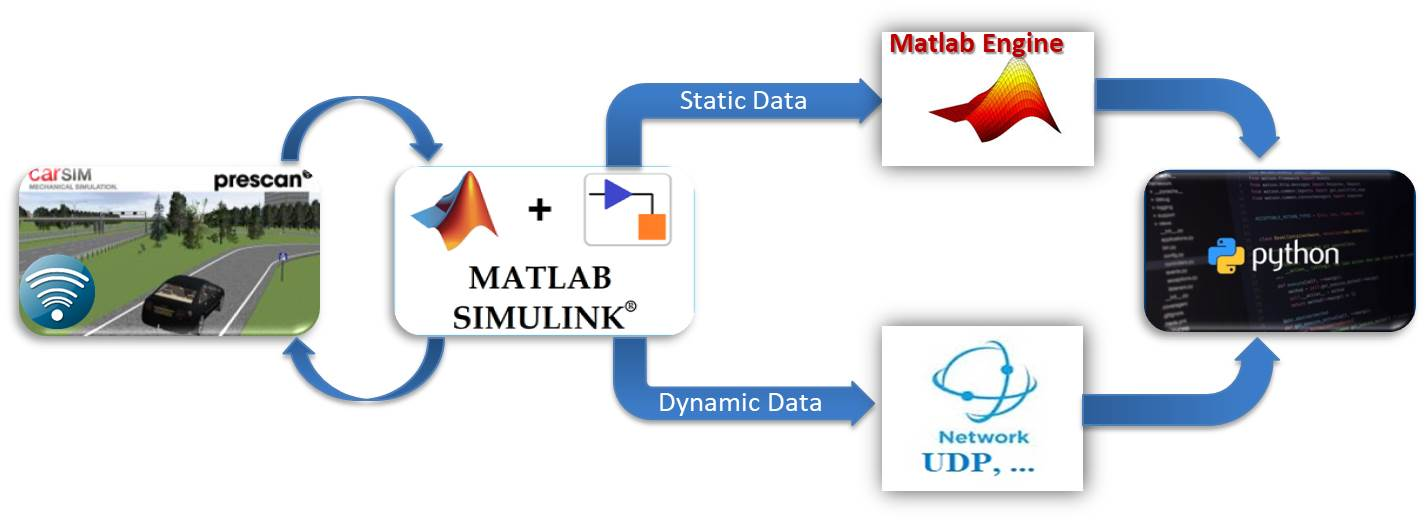
\includegraphics[width=1\linewidth]{Figures/block-diagram-white}
%	\caption{بلوک دیالگرام لایه های کلی}
%	\label{fig:block-diagram2}
%\end{figure}
%
%در شکل 
%\ref{fig:block-diagram2}
%از سمت چپ به راست اجزا یاد شده و نحوه ارتباط آن‌ها با‌یک‌دیگر را به‌خوبی نشان می‌دهد. این بلاک ها و ارتباط ها عبارتند از:
%
%\begin{itemize}
%	\item 
%	اولین بلاک آن، نرم افزار \textbf{پری‌اسکن }می‌باشد. وظیفه اصلی این نرم افزار، شبیه سازی دینامیک یک اتومبیل و یا موتور و ... می‌باشد. همچنین ایجاد یک محیط گرافیکی زیبا و یک پنل کاربری گرافیکی برای ساخت ماشین ها از دیگر حسن های این نرم افزار است.
%	
%	فایل های مهم ایجاد شده توسط این بخش، \texttt{.pex} و \texttt{.pb} می‌باشد.
%	
%	\item
%	بلاک بعدی ترکیبی از \textbf{متلب و سیمولینک }است. چرا که نرم افزار پری‌اسکن این امکان را دارد که برای کنترل و دسترسی بیشتر به قسمت های کنترلی مختلف، چیزی به نام \lr{API} ارائه می‌دهد. این \lr{API} یک فایل سیمولینک را در اختیار کابران قرار میدهد که در آن بلوک های مشخصی به یکدیگر متصل هستند و با مطالعه و تغییر آن بلوک ها می‌توان کنترل سیستم را به دست گرفت.
%	
%	فایل های مهم این بخش نیز در فرمت \texttt{.slx} و \texttt{.m} در دسترس هستند.
%	
%	همچنین \w{api} یاد شده، دستورات دیگری را جهت دریافت داده های استاتیک محیط ساخته شده در این نرم افزار را به کاربران خویش در محیط متلب می‌دهد.
%	
%	\item
%	دو بلوک بعدی، مربوط به اتصال بین متلب و یا سیمولینک با پایتون هستند. 
%	
%	بلوک بالایی این اتصال را بین داده های استاتیک شامل طول جاده و عرض هر لاین، موقعیت اولیه اتومبیل و جاده، و بسیاری اطلاعات دیگر که بسیاری از آن اطلاعات استفاده نشده اند زیرا در این پروژه مفید نبوده اند. این بلوک، فایل سیمولینک را تغییر نمی‌دهد.
%	
%	بلوک پایینی نیز با استفاده از روش های شبکه کردن، می‌تواند داده های پویا را از محیط سیمولینک به پایتون منتقل کند. این داده های پویا عبارتند از موقعیت و سرعت و اطلاعات دیگری از اتومبیل در حال حرکت، اطلاعات سنسورها و ... باشد.
%	
%	\item 
%	بلوک بعدی پایتون است که خود شامل لایه های دیگری است که در شکل 
%	\ref{fig:python-layers}
%	به تفضیل بیان شده است. نکته جالب در آن این است که در آن لایه ها اثری نیز از دو بلوک پیشین آمده است. همچنین بخش اصلی کار، یا به عبارتی مغز و هوش این کار در این قسمت توسعه یافته است.
%\end{itemize}
%




در فصل \ref{ch:rl} توضیح بسیار مختصری در مورد خود مفاهیم یادگیری تقویتی ارائه می‌شود. فصل \ref{ch:resault} راه اندازی کد و نتایج حاصل این پروژه را نشان می‌دهد. پیش از راه اندازی باید باتوجه به فصل \ref{ch:req}، پیشنیاز های نصب آن تهیه و نصب گردند. همچنین آن فصل توضیح مختصری در مورد چیستی هریک از آن پیشنیاز ها ارایه کرده است. در فصل \ref{ch:alg}، نحوه تعریف پارامترهای الگوریتم یادگیری تقویتی به صورت کامل بسط داده شده اند. فصل \ref{ch:fani}، جزییات پیاده سازی محیط شبیه سازی را نشان می‌دهد و بر روی جزییات فنی آن تمرکز دارد.











\chapter{طریقه‌ی مرجع نویسی و واژه‌نامه‌}
\section{طریقه‌ی مرجع نویسی}
برای نوشتن مراجع پایان نامه، برای راحتی کار به صورت زیر عمل می‌کنیم:
\subsection{بارگیری مراجع}
در ابتدا مراجع را باید از سایت‌های معتبر بارگیری کنیم، مثلا برای ارجاع دادن به مقاله‌ی
\lr{A classification of some Finsler connections and their applications}
ابتدا به سایت
\href{scholar.google.com}{گوگل اسکولار} 
رفته و این مقاله را جستجو می‌کنیم. پس از پیدا کردن این مقاله، مانند شکل زیر، در زیر نام و چکیده‌ی مقاله، $5$ گزینه وجود دارد که عبارتند از:\\

\begin{enumerate}
\item \lr{ Cited by}

\item \lr{ Related articles}

\item \lr{ All 6 versions}

\item \lr{ Cite}

\item \lr{ Save}
\end{enumerate}
\begin{figure}[!h]
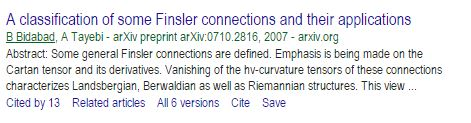
\includegraphics[height=3cm]{bidabad}
\caption{نمونه یک مقاله در گوگل اسکولار}
\end{figure}
در اینجا ما به گزینه‌ی چهارم یعنی
\lr{ Cite}
احتیاج داریم. بر روی آن کلیک کرده و پنجره‌ای مانند
\cref{fig.2}
باز می‌شود که دارای $4$ گزینه‌ی زیر است:
\begin{enumerate}
\item \lr{BibTeX}

\item \lr{EndNote}

\item \lr{RefMan}

\item \lr{RefWorks}
\end{enumerate}
\begin{figure}
\centering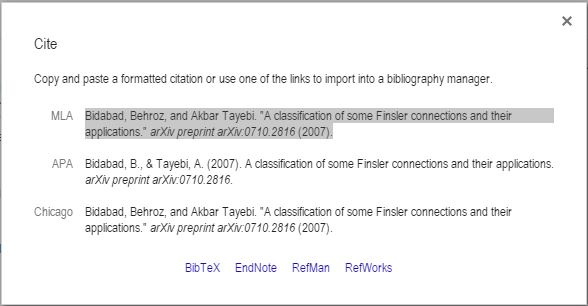
\includegraphics[scale=.6]{bibref}
\caption{پنجره‌ی باز شده در گوگل اسکولار}\label{fig.2}
\end{figure}
روی گزینه‌ی اول، یعنی
\verb;BibTeX;
کلیک کرده و همه‌ی نوشته‌های پنجره‌ی باز شده را مانند زیر، کپی کرده و در فایل
\verb;references.bib;
موجود در فایل
\verb;AUTthesis;
پیست می‌کنیم. سپس کلیدهای
\verb;Ctrl+s;
را می‌زنیم تا فایل ذخیره شود.\\
\begin{latin}
	\normalsize
\begin{verbatim}
@ article{bidabad2007classification,
title={A classification of some Finsler connections and their applications},
author={Bidabad, Behroz and Tayebi, Akbar},
journal={arXiv preprint arXiv:0710.2816},
year={2007}
}
\end{verbatim}
\end{latin}
\subsection{روش ارجاع در متن}
برای ارجاع دادن به مقاله‌ی بالا، باید در جایی که می‌خواهید ارجاع دهید، دستور زیر را تایپ کنید:
\begin{latin}
\lr{$\backslash$cite\{bidabad2007classification\}}
\end{latin}
همانطور که مشاهده می‌کنید از کلمه‌ای که در سطر اول ادرس مقاله آمده (یعنی کلمه‌ی پس از
\lr{@article$\lbrace$})
استفاده کرده‌ایم. پس از دستور فوق، به صورت \cite{bidabad2007classification} و \cite{aa} مرجع خواهد خورد. توجه شود که در صورتی مراجع چاپ خواهند شد که در متن به انها ارجاع داده شده باشد. همچنین برای ارجاع چندتایی از دستور 
\lr{$\backslash$cite\{name1, name2,...\}}
استفاده کنید که به‌صورت \cite{najafi2008finsler, zakeri, najafi} ارجاع خواهند خورد.
\subsection{روش اجرای برنامه}
ابتدا فایل
\verb;AUT_thesis.tex;
را باز کرده و آن را دو بار اجرا کنید. سپس حالت اجرا را از 
\verb;Build Quick;
به حالت
\verb;Bibtex;
تغییر داده و دوباره برنامه را اجرا کنید. دو بار دیگر برنامه را در حالت 
\verb;Build Quick;
اجرا کرده و نتیجه را مشاهده کنید. در این روش تمامی مراجع بر اساس اینکه کدام یک در متن زودتر به آن ارجع داده شده لیست خواهند شد.
\subsection{مراجع فارسی}
برای نوشتن مراجع فارسی باید به صورت دستی، در همان فایل قبلی به صورت زیر عمل می‌کنیم:
\begin{LTR}
\noindent\verb;@article{manifold,;\\
\verb;title={;منیفلد هندسه\verb;},;\\
\verb;author={;بیدآباد دکتربهروز \verb;},;\\
\verb;journal{; امیرکبیر صنعتی دانشگاه\verb;},;\\
\verb;year={1389},;\\
\verb;LANGUAGE={Persian};\\
\verb;};
\end{LTR}
همانطور که مشاهده می‌کنید تنها تفاوت آن با حالت مراجع انگلیسی، سطر آخر آن می‌باشد که زبان را مشخص می‌کند که حتماً باید نوشته شود.
\section{راهنمای واژه‌نامه}

به دلیل پیچیدگی واژه‌نامه‌های موجود در سایت پارسی لاتک، از روش زیر برای نوشتن واژه‌نامه استفاده کنید:

ابتدا با استفاده از اکسل، واژه های خود را یک‌بار براساس حروف الفبای فرسی و بار دیگر انگلیسی مرتب کنید. سپس واژه ها را در فایل \lr{dicen2fa} و \lr{dicfa2en} قرار دهید.

\section{ساخت نمایه}\label{Namaye}
\subsection{ساخت نمایه}
 \begin{enumerate}

\item
کلمات مورد نظر خود مثلا \lr{word} با دستور \verb|\index{word}| ایندکس کنید.
\item
نحوه‌ی اجرای \lr{Make Index}   در ویرایشگرهای \lr{TeX Maker} و \lr{TeX Works}:
\begin{itemize}
\item  تک‌میکر: از منوی \lr{Tools} گزینه‌ی \lr{Xindy Make Index} را کلیک کنید یا از دکمه‌‌های میانبر \lr{Ctrl+Alt+I} استفاده کنید.

\item  تک‌ورکز: ابتدا باید مثل عکس زیر تنظیم  و سپس گزینه‌ی \lr{Xindy Make Index}  انتخاب و روی دکمه‌ی سبز رنگ کلیک کنید یا از دکمه‌های  \lr{Ctrl+T} استفاده کنید.

\begin{figure}[!h]
\centerline{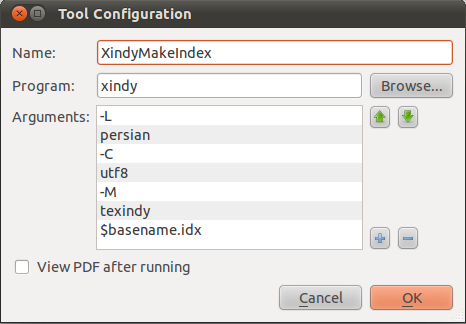
\includegraphics[width=.5\textwidth]{Xindy_Make_Index.png}}
\caption{تنظیمات مربوط به تک‌ورکز}
\end{figure}

\end{itemize}
 \end{enumerate}
 
 \index{کتاب}
\index{پارسی‌لاتک}
\index{بی‌دی}
\index{سوال}
\index{عنصر}
\index{گزینه}
\index{ژاکت}
\index{مرکز دانلود}
\index{اجرا}
\index{تک‌لایو}
\index{ثالث}
\index{جهان}
\index{چهار}
\index{حمایت}
\index{خواهش}
\index{دنیا}
\index{زی‌پرشین}
\index{ریحان}
\index{شیرین}
\index{صمیمی}
\index{ضمیر}
\index{طبیب}
\chapter{جزئیات فنی پروژه}


\section{مقدمه}
در این پروژه از جهت آنکه نسخه قبلی و پیشینی برای  آن نبوده است، به ناچار می‌بایست که کد آن از صفر تا صد آن به صورت دستی نوشته شود. از این‌رو، پیچیدگی های بسیار فراوان را به طور خاص در پی داشت. ابزار های زیادی نیز بنابه شرایط در آن استفاده شد که ارتباط بین آن ابزار ها و اجزا، بر این پیچیدگی پیاده سازی طرح افزوده بود.

ابزار های اصلی و کلی که در این پروژه استفاده شده بود، عبارتند از:

\begin{itemize}
	\item 
	\textbf{نرم افزار پری اسکن}
	\LTRfootnote{PreScan}
	، نسخه \lr{$8.5.0$}
	
	\item 
	\textbf{نرم افزار قدرتمند متلب}
	\LTRfootnote{Matlab}
	، نسخه \lr{R2017b}
	\item 
	\textbf{زبان برنامه نویسی پایتون}
	، نسخه \lr{$3.6.9$}
\end{itemize}

بنابراین برای راه اندازی مجدد کد این پروژه لازم است که موارد بالا روی کامپیوتر شخص به صورت کامل نصب باشد.

همچنین لازم به ذکر است که برخی ابزارات دیگر نیز در این پروژه استفاده شده است که احتمالا با نصب موارد بالا دیگر نیازی به نصب آن ها به صورت جداگانه نیست. هدف این ابزار ها ایجاد اتصال بین اجزای اصلی گفته شده است. این گروه شامل موارد زیر هستند:

\begin{itemize}
	\item 
	\textbf{سیمولینک}
	\LTRfootnote{Simulink}
	، جهت اتصال بین متلب و پری اسکن
	
	\item 
	\textbf{شبکه \lr{UDP}}
	\RTLfootnote{برای این منظور از ماژول \lr{socket} در پایتون استفاده شده است. }
	، جهت اتصال داده های پویا 
	\LTRfootnote{Dynamic Data}
	بین پایتون و سیمولینک
	
	\item 
	\textbf{موتور متلب}
	\LTRfootnote{\matlabengine}
	، جهت اتصال داده های ساکن
	\LTRfootnote{Static Data}
	بین پایتون و سیمولینک
\end{itemize}

در این فصل جزئیات بیشتری در مورد لزوم و دلیل استفاده از این ابزار ها بررسی می‌شود.


\section{دورنمای کلی طرح}
همان‌طور که گفته شد، در این پروژه از ابزار های مختلفی استفاده شده است. برخی ابزارات دیگر نیز جهت ایجاد اتصال بین آن ابزار ها استفاده شده اند. در این بخش، این اجزا به تفصیل بررسی خواهد شد.
 
 هر کدام از این اجزا کار مشخصی را بر عهده دارند.
 شکل  
\ref{fig:block-diagram}
این ارتباط را نشان می‌دهد.

\begin{figure}[h!]
	\centering
	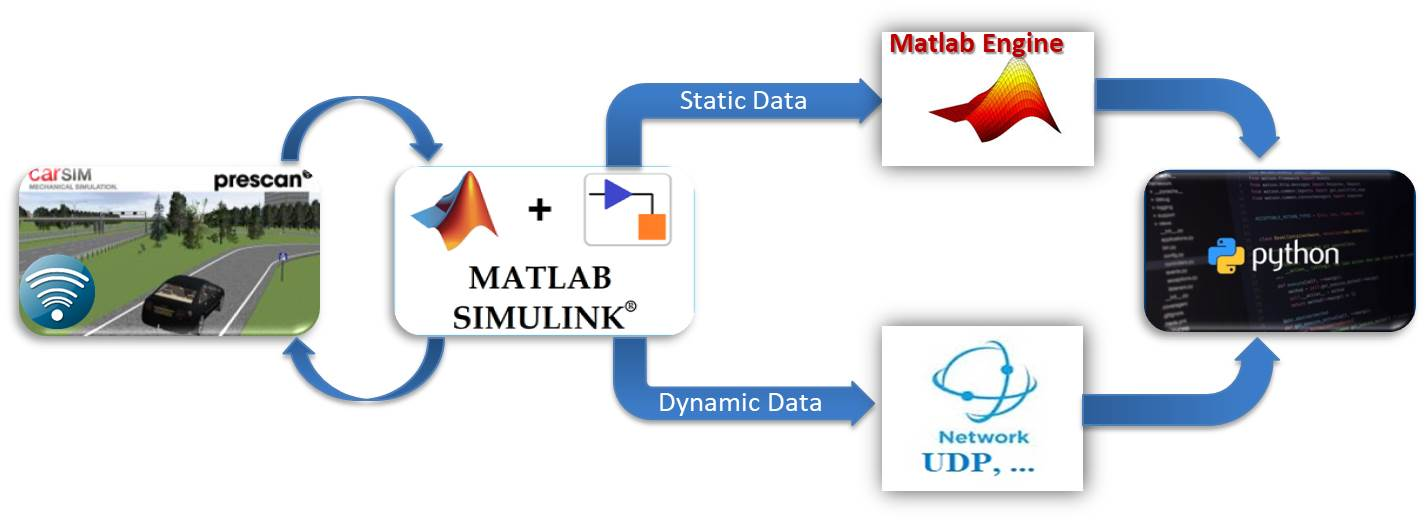
\includegraphics[width=1\linewidth]{Figures/block-diagram-white}
	\caption{بلوک دیالگرام لایه های کلی}
	\label{fig:block-diagram}
\end{figure}

در شکل 
\ref{fig:block-diagram}
از سمت چپ به راست اجزا یاد شده و نحوه ارتباط آن‌ها با‌یک‌دیگر را به‌خوبی نشان می‌دهد. این بلاک ها و ارتباط ها عبارتند از:

\begin{itemize}
	\item 
	اولین بلاک آن، نرم افزار \textbf{پری‌اسکن }می‌باشد. وظیفه اصلی این نرم افزار، شبیه سازی دینامیک یک اتومبیل و یا موتور و ... می‌باشد. همچنین ایجاد یک محیط گرافیکی زیبا و یک پنل کاربری گرافیکی برای ساخت ماشین ها از دیگر حسن های این نرم افزار است.
	
	فایل های مهم ایجاد شده توسط این بخش، \texttt{.pex} و \texttt{.pb} می‌باشد.
	
	\item
	بلاک بعدی ترکیبی از \textbf{متلب و سیمولینک }است. چرا که نرم افزار پری‌اسکن این امکان را دارد که برای کنترل و دسترسی بیشتر به قسمت های کنترلی مختلف، چیزی به نام \lr{API} ارائه می‌دهد. این \lr{API} یک فایل سیمولینک را در اختیار کابران قرار میدهد که در آن بلوک های مشخصی به یکدیگر متصل هستند و با مطالعه و تغییر آن بلوک ها می‌توان کنترل سیستم را به دست گرفت.
	
	فایل های مهم این بخش نیز در فرمت \texttt{.slx} و \texttt{.m} در دسترس هستند.
	
	همچنین \api یاد شده، دستورات دیگری را جهت دریافت داده های استاتیک محیط ساخته شده در این نرم افزار را به کاربران خویش در محیط متلب می‌دهد.

	\item
	دو بلوک بعدی، مربوط به اتصال بین متلب و یا سیمولینک با پایتون هستند. 
	
	بلوک بالایی این اتصال را بین داده های استاتیک شامل طول جاده و عرض هر لاین، موقعیت اولیه اتومبیل و جاده، و بسیاری اطلاعات دیگر که بسیاری از آن اطلاعات استفاده نشده اند زیرا در این پروژه مفید نبوده اند. این بلوک، فایل سیمولینک را تغییر نمی‌دهد.
	
	بلوک پایینی نیز با استفاده از روش های شبکه کردن، می‌تواند داده های پویا را از محیط سیمولینک به پایتون منتقل کند. این داده های پویا عبارتند از موقعیت و سرعت و اطلاعات دیگری از اتومبیل در حال حرکت، اطلاعات سنسورها و ... باشد.
	
	\item 
	بلوک بعدی پایتون است که خود شامل لایه های دیگری است که در شکل 
	\ref{fig:python-layers}
	به تفضیل بیان شده است. نکته جالب در آن این است که در آن لایه ها اثری نیز از دو بلوک پیشین آمده است. همچنین بخش اصلی کار، یا به عبارتی مغز و هوش این کار در این قسمت توسعه یافته است.
\end{itemize}
\subsection{تقسیم بندی وظایف هر بخش}
بخش اصلی کار که وظیفه آن تصمیم گیری و انتخاب مسیر درست توسط یک عامل
\LTRfootnote{Agent}
(که در این پروژه، عامل همان اتومبیل می‌باشد) در پایتون انجام می‌شود. وظیفه اصلی بخش متلب و سیمولینک و پری‌اسکن، ایجاد یک محیط شبیه سازی است. 

\begin{note}


این محیط شبیه سازی اهمیت زیادی در الگوریتم های یادگیری تقویتی دارد. زیرا در این الگوریتم ها یک «عامل» با «محیط
\LTRfootnote{Environment}
» در تعامل است. تعامل در این الگوریتم ها به معنای این است که «عامل» در یک «حالت
\LTRfootnote{State}
» قرار دارد. سپس متناسب با آن یک «حرکت
\LTRfootnote{Action}
» انجام می‌دهد. با این «حرکت»، «محیط» به آن یک مقدار «امتیاز» و یک «حالت» جدید بر‌می‌گرداند. 
بنابراین داشتن یک محیط شبیه سازی کامل و دقیق از اجزای ضروری کار است.

\end{note}

بخش های دیگر مربوط به ارتباط این قسمت ها به یک‌دیگر بودند که پیچیدگی های زیادی را رقم زده است.

به طور ساده‌تر و کلی‌تر می‌توان گفت که پایتون نقش «عامل» و پری‌اسکن نقش «محیط» را دارد.

\section{معرفی نرم افزار پری‌اسکن}
می‌توان در ابتدا گفت که این نرم‌افزار یک افزونه متلب و سیمولینک است اما توانایی زیادی که آن دارد باعث می‌شود که بگوییم این محصول از متلب و سیمولینک جعت رسیدن به هدف خود کمک می‌گیرد.

نرم افزار پری‌اسکن یکی از نرم افزار های بسیار قدرتمند در زمینه شبیه سازی مسایل مربوط به وسایل نقلیه است که می‌تواند حرکت یک ویله نقلیه را به طور خیلی دقیق و مناسب شبیه سازی کند. همچنین در کنار این وظیفه مهم، یک محیط گرافیکی مناسب را در اختیار کاربران خود قرار می‌دهد که از دیگر حسن های آن است.
شکل 
\ref*{fig:prescan-gallery} این توانایی ها را به تصویر کشیده است.
 
همچنین این نرم افزار یک سری فایل خروجی به کاربر می‌دهد که یکی از فایل های آن فایل سیمولینک است که اجازه تغییر و دسترسی به داخل برخی بلاک ها به ما کمک می‌کند که اطلاعات خود را از دل آن نرم افزار بیرون بکشیم.
\RTLfootnote{جهت کسب اطلاعات بیشتر و تهیه این نرم افزار به لینک زیر مراجعه کنید:
\\
\lr{\href{https://tass.plm.automation.siemens.com/prescan}{https://tass.plm.automation.siemens.com/prescan}}
}

از این رو در مقابسه با محیط های دیگر، محاسن زیادی را داشت که هدف این پروژه را در به کار‌گیری این ابزار تحت تاثیر قرار داد.



\begin{figure}
	\centering
	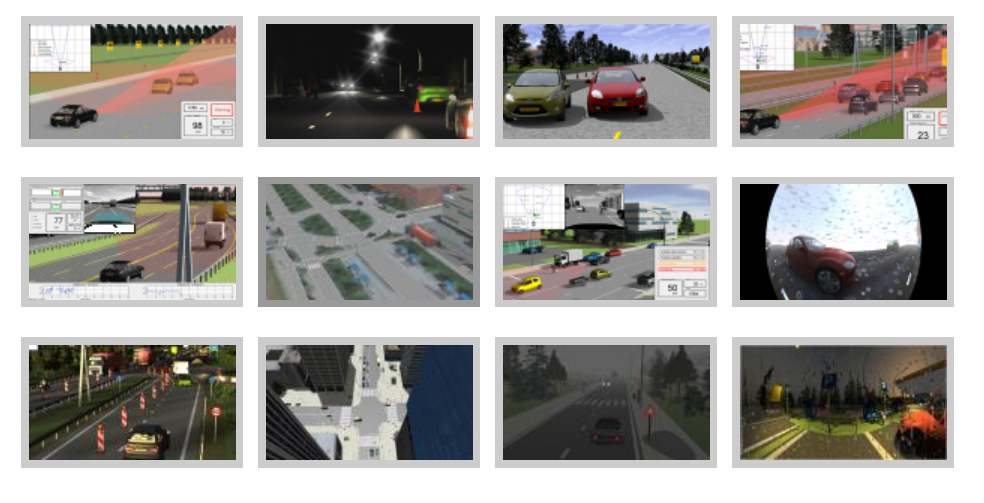
\includegraphics[width=0.8\linewidth]{Figures/Prescan-gallery}
	\caption{بخشی از توانایی های نرم افزار پری‌اسکن در شبیه سازی}
	\label{fig:prescan-gallery}
\end{figure}





\subsection{بخش های مختلف نرم افزار پری‌اسکن}
پس از دانلود و نصب نسخه \lr{8.5.0} این نرم‌افزار چهار آیکون مانند شکل 
\ref{fig:prescan-icons}
به محیط دسکتاپ اضافه می‌کند.  اصلی ترین آن ها 
\lr{PreScan Proccess Manager 8.5.0}
نام دارد.

\begin{figure}[h]
	\centering
	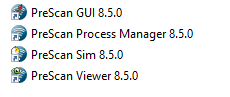
\includegraphics[width=0.4\linewidth]{Figures/prescan-icons}
	\caption{آیکون های اضافه شده بر روی محیط دسکتاپ پس از نصب پری‌اسکن}
	\label{fig:prescan-icons}
\end{figure}
 
 با انتخاب آن صفحه ای مانند زیر باز می‌شود.

\begin{figure}[h]
	\centering
	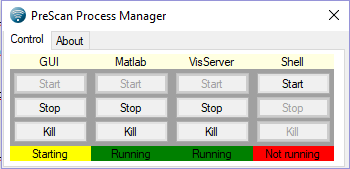
\includegraphics[width=0.5\linewidth]{Figures/Prescan-panel}
	\caption{پنل مدریت نرم‌افزار پری‌اسکن}
	\label{fig:prescan-panel}
\end{figure}

این پنجره شامل گزینه های زیر است:
\begin{multicols}{2}
\begin{itemize}
	\item \lr{GUI}
	\item \lr{VisServer}
	\item \lr{Matlab}
	\item \lr{Shell}
\end{itemize}
\end{multicols}

برای ایجاد یک محیط جدید باید \lr{GUI} را استارت کرد. پس از مدتی صفحه ای مانند شکل 
\ref{fig:prescan-gui}
باز می‌شود. 





\begin{figure}
	\centering
	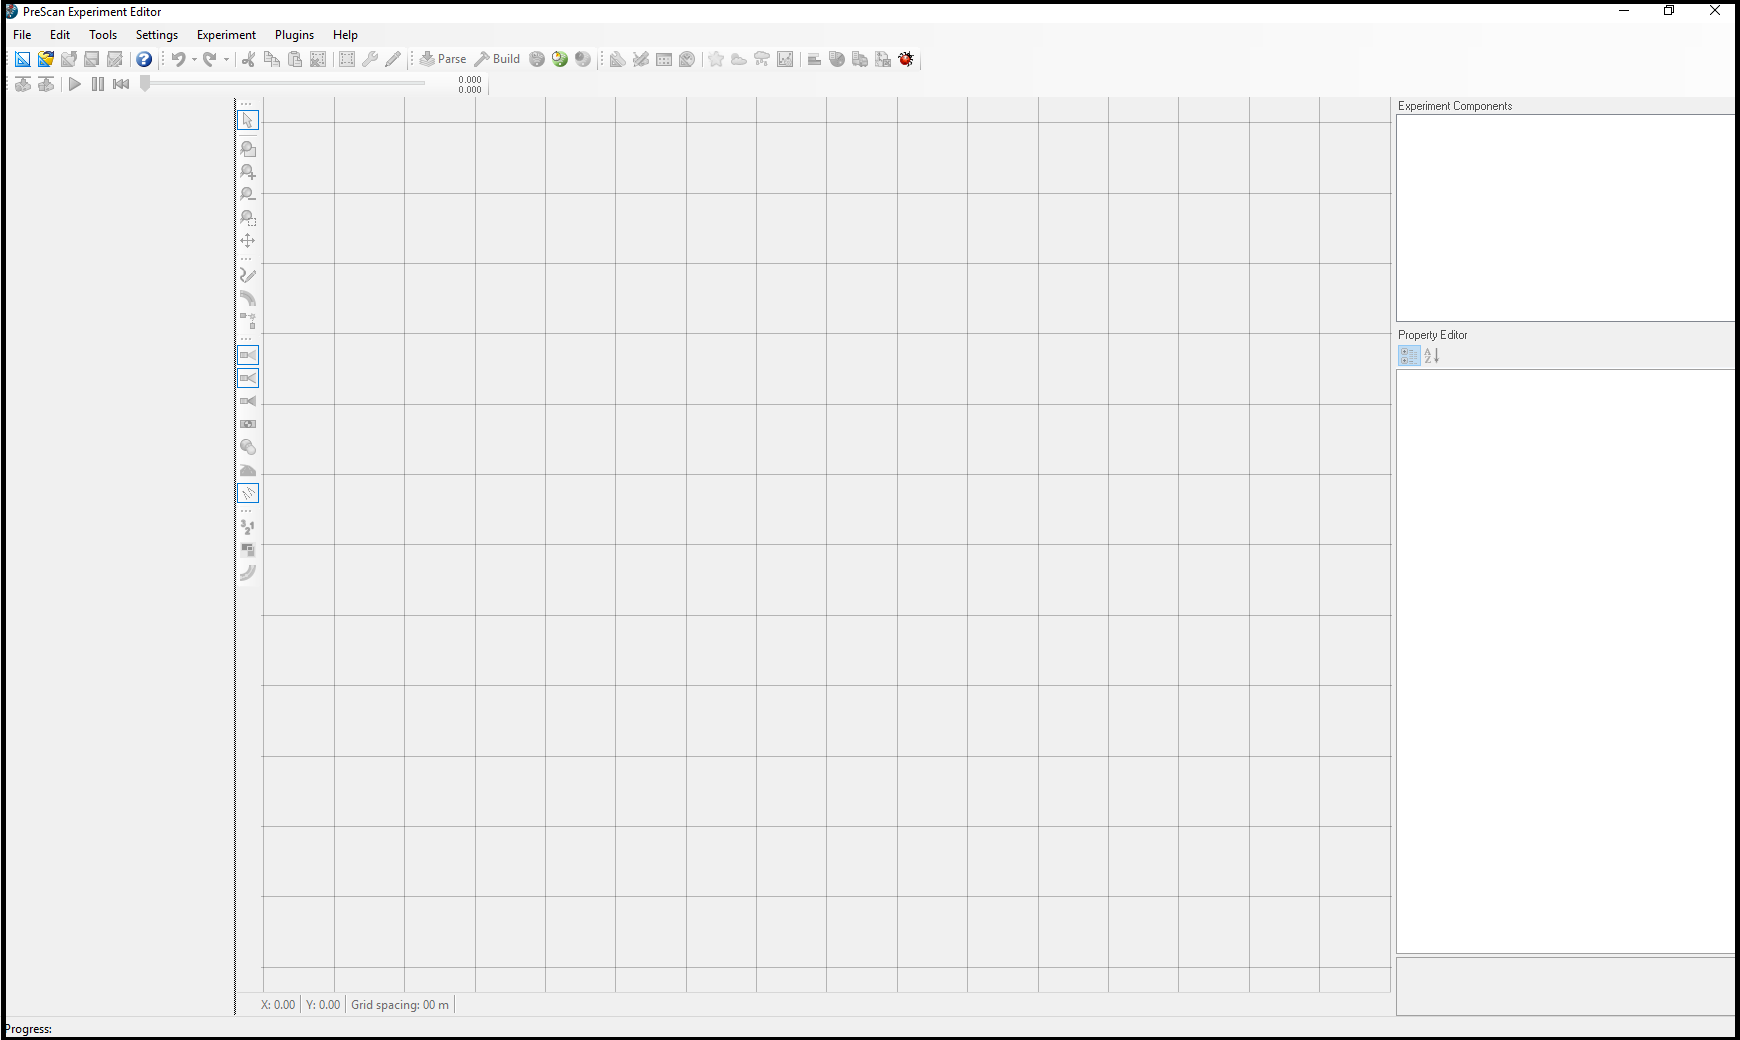
\includegraphics[width=0.7\linewidth]{Figures/Prescan-GUI}
	\caption{صفحه گرافیکی محیط پری‌اسکن}
	\label{fig:prescan-gui}
\end{figure}



پس از ایجاد مدل ها و ذخیره آن، فایل های \texttt{**.pex} و \texttt{**.pb} و \texttt{**\_cs.slx} ساخته می‌شود.
\RTLfootnote{علامت ** به معنای یک اسم مشترک در این سه فایل استفاده شده است. }

جهت استفاده از فایل سیمولینک باید در شکل 
\ref{fig:prescan-panel}
متلب را استارت کنید.
\begin{remark}
	برای اجرای فایل های سیمولینک خروجی، لازم است که متلب را فقط و فقط با استفاده از نرم افزار پری‌اسکن و با استفاده از پنل مدیریت نرم افزار معرفی شده در شکل 
	\ref{fig:prescan-panel}
	باز شود. در صورتی که به صورت مستقیم این کار انجام شود، به مشکل منتهی می‌شود.
\end{remark}


دو قسمت دیگر نیز در شکل 
\ref{fig:prescan-panel}
وجود دارد که نیازی به استارت کردن آن ها نیست و خودشان در صورت لزوم به صورت خودکار فراخوانی می‌شوند.


\subsection{فرمت های فایل های خروجی}
نرم‌افزار پری‌اسکن پس از ایجاد یک محیط جدید، فایل ها و پوشه های بسیار زیادی را ایجاد می‌کند. اما در خارج آن پوشه ها ۳ فایل وجود دارد که پسوند آن ها \texttt{**.pex} و \texttt{**.pb} و \texttt{**\_cs.slx} می‌باشد. علامت ** همان اسم پروژه‌ای است که ایجاد کرده ایم. هر یک از این فایل ها به یک بلوک از شکل 
\ref{fig:block-diagram}
مربوط می‌شود.

\begin{table}[h!]
\tableset{
%{\setcellgapes{0.5em}\makegapedcells
\begin{tabular}{|C{0.15\linewidth}|p{0.8\linewidth}|}
	\hline\rowcolor{lightgray}
	فرمت فایل
	&
	توضیحات 
	\\\hline\hline
	\texttt{**.pex} &	این فایل مربوط به اولین بلوک شکل
	\ref{fig:block-diagram}
	است و ارتباط مستقیم با \lr{GUI} دارد. برای تغییر محیط گرافیکی باید این فایل را باز کرد.
	\\ \hline   
	\texttt{**.pb} & این فایل برخی از اطلاعات فایل 
	\texttt{**.pex}
	را در اختیار دارد و با تغییر آن فایل این فایل نیز عوض می‌شود. این فایل حاوی اطلاعات استاتیک محیط ایجاد شده است و مهم ترین کاربرد آن در بلوک موتور متلب که در شکل 
	\ref{fig:block-diagram}
	نشان داده شده است می‌باشد. پایتون از طریق این فایل این اطلاعات را دریافت می‌کند.
	\\\hline
	\texttt{**\_cs.slx} &
	این فایل سیمولینک است که برای کار کردن با آن باید از پنل مدیریت شکل
	\ref{fig:prescan-panel}
	استفاده کرد. این فایل پس از ایجاد از فایل 
	\texttt{**.pex}
	مستقل می‌شود. این فایل خود قابلیت تغییر دارد و می‌توان بلوک‌های آن‌را در محیط سیمولینک تغییر داد و بلوک های دیگری به آن افزود.  در صورتی که فایل \texttt{**.pex} تغییر کند، این امکان را نیز دارد که از داخل خود سیمولینک با فشردن دکمه ای این تغییرات جدید اعمال شود بدون آن که به تغییرات خود کاربر لطمه ای وارد شود. در این پروژه این فایل، تغییرات بسیاری را تجربه کرد.
	\\\hline
\end{tabular}}
\caption{توضیحات فرمت فایل خروجی}
\label{tab:prescan-format}
\end{table}



جدول
\ref{tab:prescan-format}
توضیحات لازم را جهت آشنایی با این خروجی ها آورده است.

همچنین در بخش  
\ref{ch:fani|sec:simulink}
در مورد فایل \texttt{**\_cs.slx} توضیحات دقیق‌تری در مورد جزییات آن گفته خواهد شد.

\section{بررسی دقیق‌تر فایل سیمولینک}\label{ch:fani|sec:simulink}

فایل سیمولینک ایجاد شده توسط نرم افزار پری‌اسکن، قابلیت تغییر به دست کاربر را دارد. شکل 
\ref{fig:simulink-firstview}
فایل تغییر‌یافته مربوط به این پروژه را نشان می‌دهد.


\begin{figure}
	\centering
	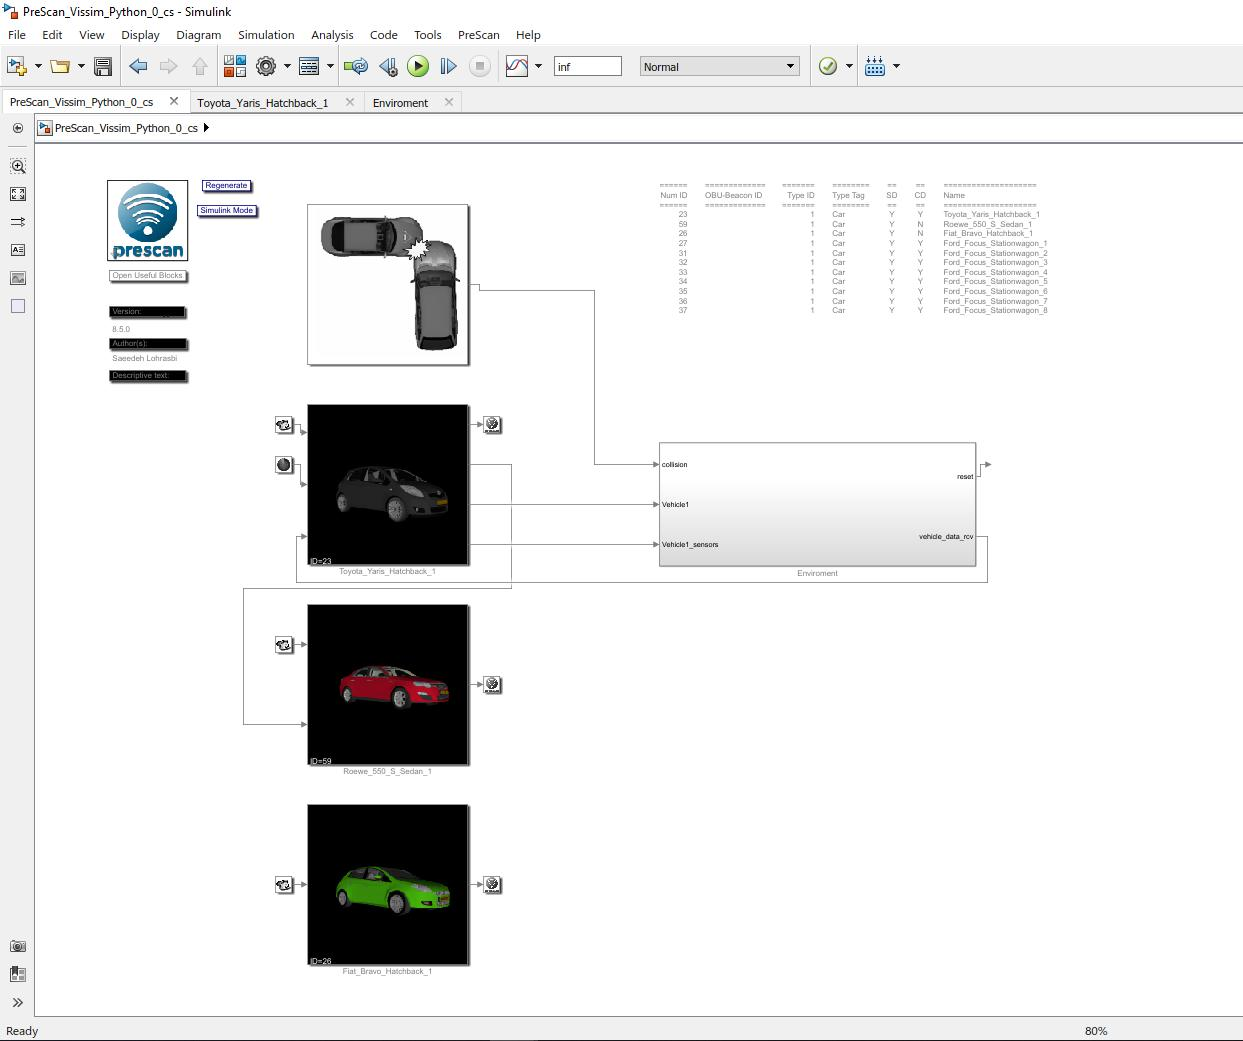
\includegraphics[width=0.7\linewidth]{Figures/simulink/first_view}
	\caption{فایل سیمولینک ایجاد شده توسط نرم افزار پری‌اسکن همراه با تغییرات}
	\label{fig:simulink-firstview}
\end{figure}




بلوک های سمت راست نشان داده شده در سمت راست شکل
\ref{fig:simulink-firstview}
توسط نرم افزار پری اسکن ایجاد شده است که البته دست‌خوش تغییراتی نیز بوده اند. 

در صورتی که با استفاده از محیط گرافیکی \lr{GUI} فایل \texttt{**.pex} تغییر کند، فایل سیمولینک تغییر نمی‌کند. در برخی موارد این تغییرات ممکن است منجر به پیغام خطا شود.

\begin{remark}\label{remark:Regenerate}
	در صورتی که فایل
	 \texttt{**.pex}
	 تغییر کند، برای اعمال این تغییرات، باید روی کلمه 
	 \lr{Regenerate}
	 که در شکل 
	 \ref{fig:simulink-generate}
	 آمده است، کلیک کرد. با این کار، تغییرات جدید اعمال می‌شود بی‌آن‌که تغییرات کاربر تحت تاثیر قرار بگیرد.
\end{remark}

\begin{figure}
	\centering
	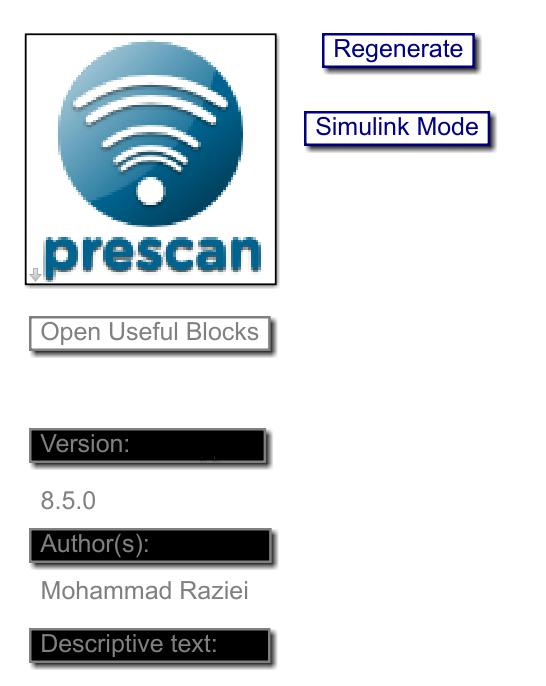
\includegraphics[width=0.4\linewidth]{Figures/simulink/generate}
	\caption{روش صحیح اعمال تغییرات روی فایل سیمولینک}
	\label{fig:simulink-generate}
\end{figure}

در شکل 
\ref{fig:simulink-generate}
همانطور که در نکته
\ref{remark:Regenerate} 
به آن اشاره شد، دکمه ای تحت عنوان 
\lr{Regenerate}
وجود دارد که استفاده از آن در همان نکته مشخص شده است. همچنین در این تصویر در زیر لوگوی برنامه پری‌اسکن، اطلاعاتی مانند شماره نسخه نرم افزار (که در این‌جا \lr{8.5.0} می‌باشد.)، نام نویسنده مشاهده می‌شود.

در شکل 
\ref{fig:simulink-firstview}
اولین بلوک سمت راست همان ماشینی است که ما آن‌را تحت کنترل گرفته‌ایم. اگه به آن وارد شویم، شکل 
\ref{fig:simulink-agent}
را مشاهده می‌کنیم.
در این تصویر ورودی و خروجی ها نقش خیلی مهمی دارند. این اطلاعات در جدول
\ref{tab:simuink-agent-io}
 آمده‌اند.



\begin{figure}[h!]
	\centering
	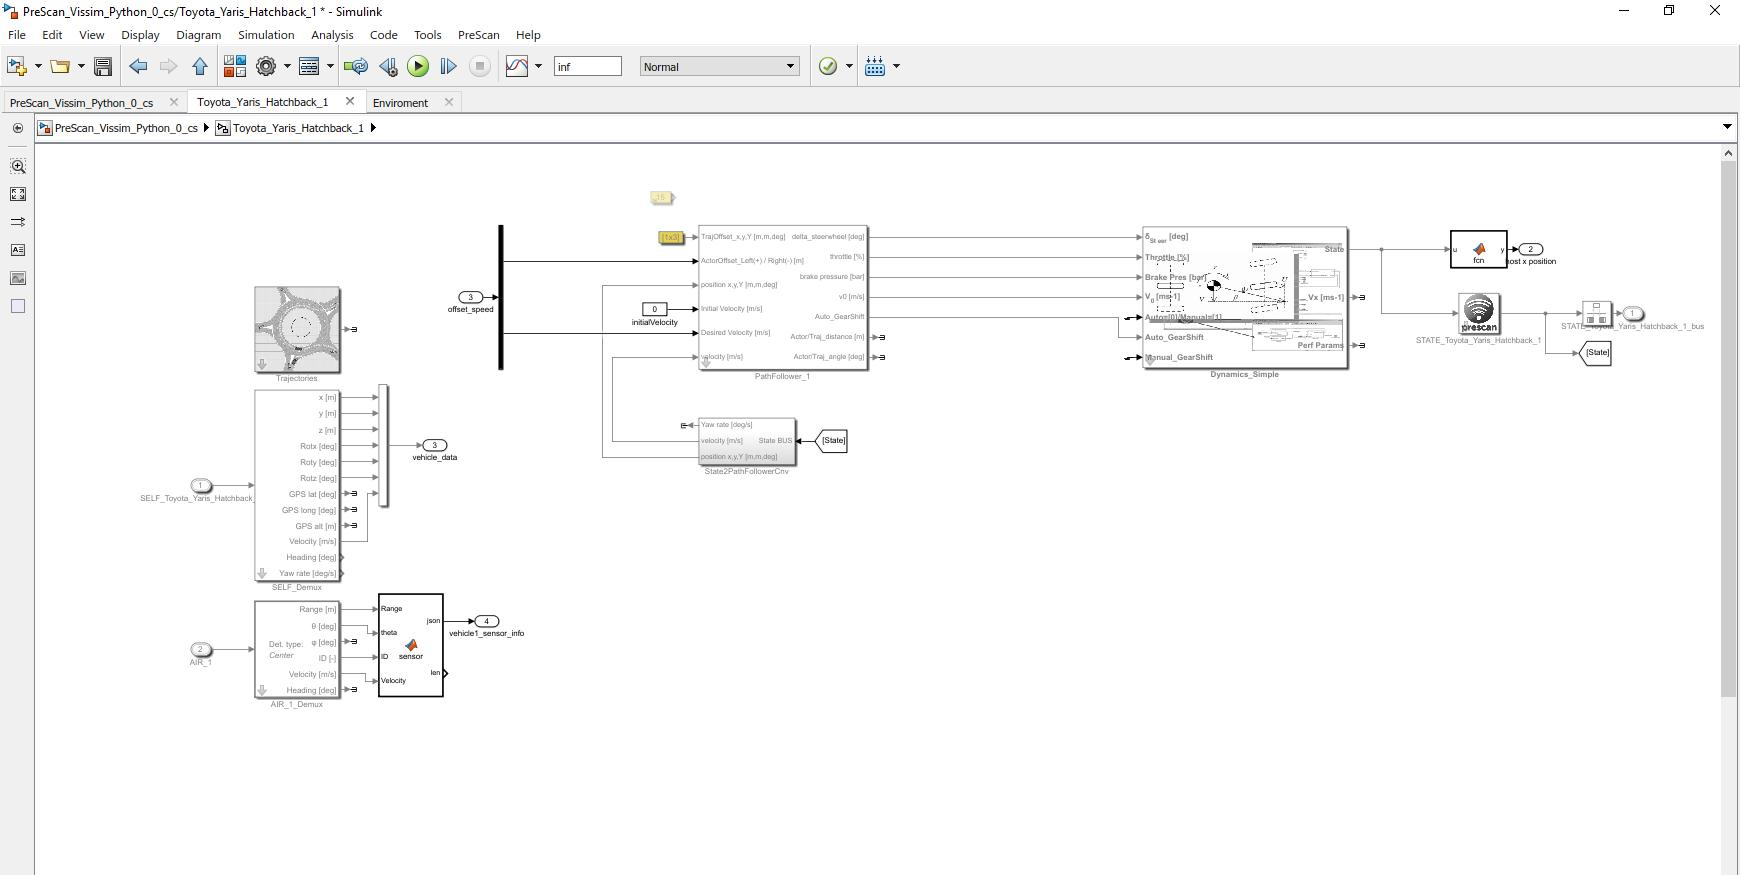
\includegraphics[width=1\linewidth]{Figures/simulink/agent}
	\caption{فایل سیمولینک - شبیه سازی اتومبیل}
	\label{fig:simulink-agent}
\end{figure}


\begin{table}[h!]
	\tableset{
		\begin{tabular}{|C{0.08\linewidth}|C{0.23\linewidth}|C{0.17\linewidth}|p{0.43\linewidth}|}
			\hline\rowcolor{lightgray}
			نوع & عنوان & بلوک مربوط & توضیحات
			\\\hline\hline
			خروجی &اطلاعات ماشین & \lr{SELF\_Demux} & اطلاعات ماشین، شامل اطلاعات موقعیت($x$،$y$ و$z$) و اطلاعات چرخش (حول $x$،$y$ و$z$) به همراه سرعت ماشین را خروجی می‌دهد. این 7 داده قبل از خروجی توسط یک \lr{mux} با یکدیگر ادغام می‌شوند.
			\\\hline
			خروجی& اطلاعات سنسور ماشین & \lr{AIR\_1\_Demux}  & اطلاعات سنسور \lr{V2C} را خروجی می‌دهد. از آنجا که این سنسور فاصله و زاویه و ...  تا ده ماشین نزدیک خود را می‌دهد. بنابراین هر‌یک از این اطلاعات یک بردار ده تایی است. برای فرستادن آن اطلاعات به خروجی، ابتدا آن‌ها را به  طریقی به فرمت جیسون
			\footnotemark%{json}
			تبدیل می‌کند و یک رشته کاراکتر با طول مشخص
			\footnotemark%{بعدا خواهید دید که مشخص بودن طول بسیار بسیار اهمیت دارد!}
			را خروجی می‌دهد.
			\\\hline
			ورودی & کنترل لاین و سرعت ماشین & \lr{PathFollower\_1} & دستورات کنترلی اتومبیل، شامل کدام خط بودن و مقدار سرعت نهایی، به صورت ورودی وارد یک \lr{demux} می‌شود و پس از جدا سازی، به بلوک مربوط متصل می‌شود.
			\\\hline
	\end{tabular}}
	\caption{بررسی ورودی ها و خروجی های مهم در شکل \ref{fig:simulink-agent}}
	\label{tab:simuink-agent-io}
\end{table}
\LTRfootnotetext[14]{json}
\RTLfootnotetext{بعدا خواهید دید که مشخص بودن طول بسیار بسیار اهمیت دارد!}


\subsection{معرفی بلوک 
\lr{Environment}
و بررسی جزییات آن
}

در جدول \ref{tab:simuink-agent-io} صرفا ورودی خروجی های مهم مورد بررسی قرار گرفته است. این ورودی ها و خروجی های مهم به یک بلوک دیگر منتقل می‌شود. بلوک 
\lr{Environment}
همان بلوک است که در شکل
\ref{fig:simulink-firstview}
نیز مشخص است و در شکل 
\ref{fig:simulink-env}
نیز از زاویه نزدیک تر با جزییات بیشتر می‌توان آن‌را مشاهده نمود.
%\code[matlab]{simulink-json-sensor.m}



\begin{figure}
	\centering
	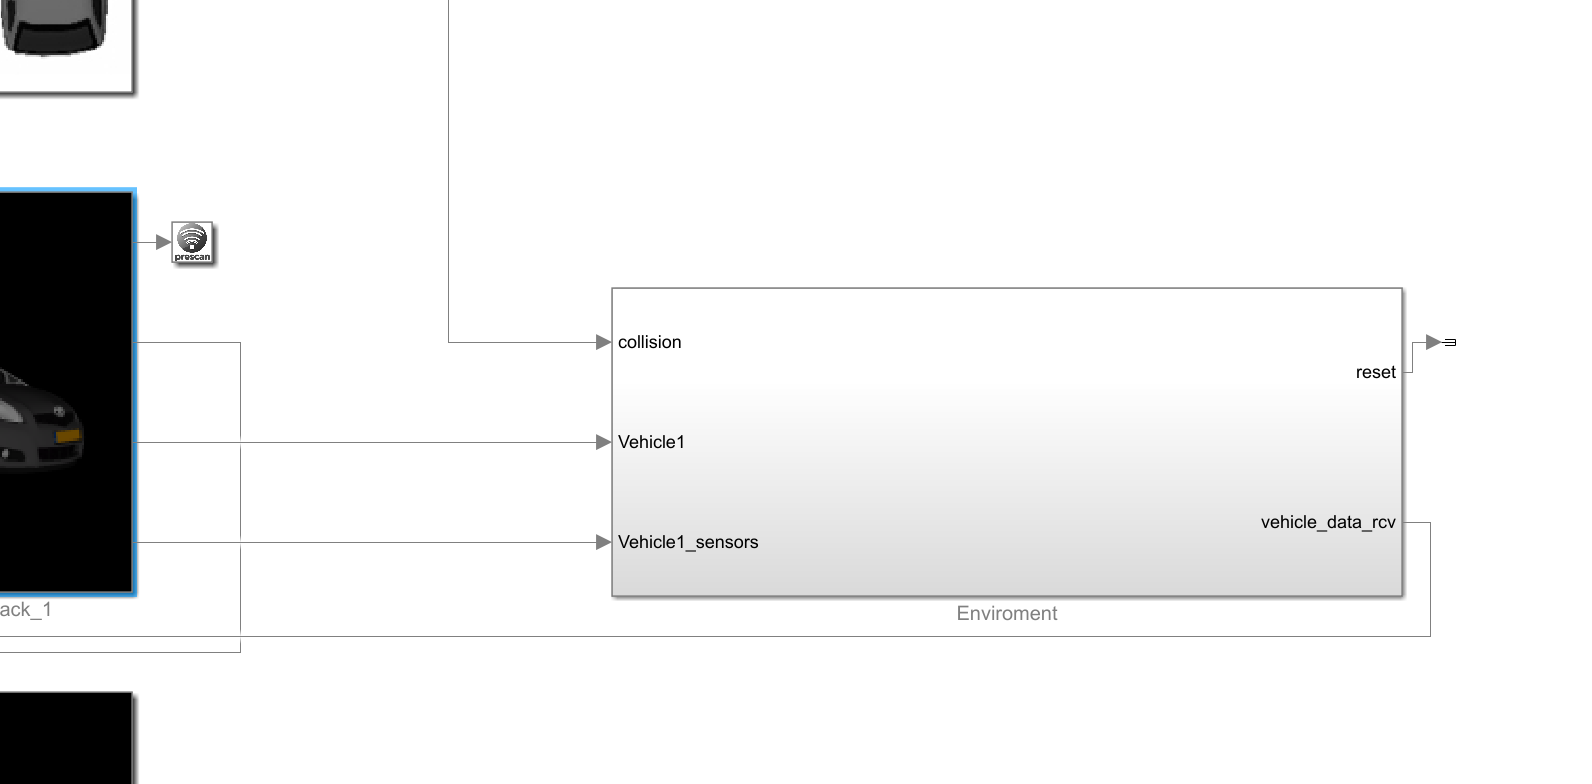
\includegraphics[width=0.7\linewidth]{Figures/simulink/simulink-Env}
	\caption{نگاهی از نزدیک به بلوک \lr{Environmnet}}
	\label{fig:simulink-env}
\end{figure}




وظیفه اصلی بلوک 
\lr{Environment}
جمع آوری اطلاعات محیط سیمولینک و همچنین ارسال دستورات کنترلی به آن هاست. اطلاعات جمع آوری شده از محیط سیمولینک شامل موارد زیر است.

\begin{itemize}
	\item 
	اطلاعات ماشینی که نقش «عامل» را در الگوریتم دارد.
	\item 
	اطلاعات سنسور های ماشین «عامل»
	\item 
	اطلاعات مربوط به تصادف کردن و کدوم ماشین با کدوم ماشین تصادف کرده است.	
\end{itemize}

این اطلاعات به صورت ورودی به این بلوک وارد می‌شود و دستورات کنترلی شامل کنترل لاین ماشین به همراه مقدار سرعت نهایی ماشینی که نقش «عامل» در الگوریتم دارد، از این بلوک خارج می‌شود.

پیشتر صحبت شد که وظیفه تصمیم گیری بر عهده کد پایتون است. با این حساب سیمولینک قدرت تشخیص و تصمیم گیری ندارد. از این رو وظیفه بلوک 
\lr{Environment}
نیز تصمیم گیری نمی‌باشد بلکه با تکنیک هایی سعی بر برقراری ارتباط با کد پایتون دارد. در حقیقت این بلوک نقش واسط بین سیمولینک و پایتون را دارد. این بلوک علاوه بر دستورات کنترلی لاین و سرعت، دستور «شروع کردن دوباره» و یا ریست را نیز دریافت می‌کند. با این دستور تمامی اطلاعات به حالت اول بر خواهد گشت و ماشین «عامل» به جای اول بر خواهد گشت و منتظر دستورات جدید می‌ماند.

شکل 
\ref{fig:block-diagram}
توضیح بسیار کلی  در مورد این نحوه ارتباط نشان داده است و در شکل 
\ref{fig:inside-environment}
جزییات بیشتری را در مورد داخل این بلوک را نشان می‌دهد.


\begin{figure}
	\centering
	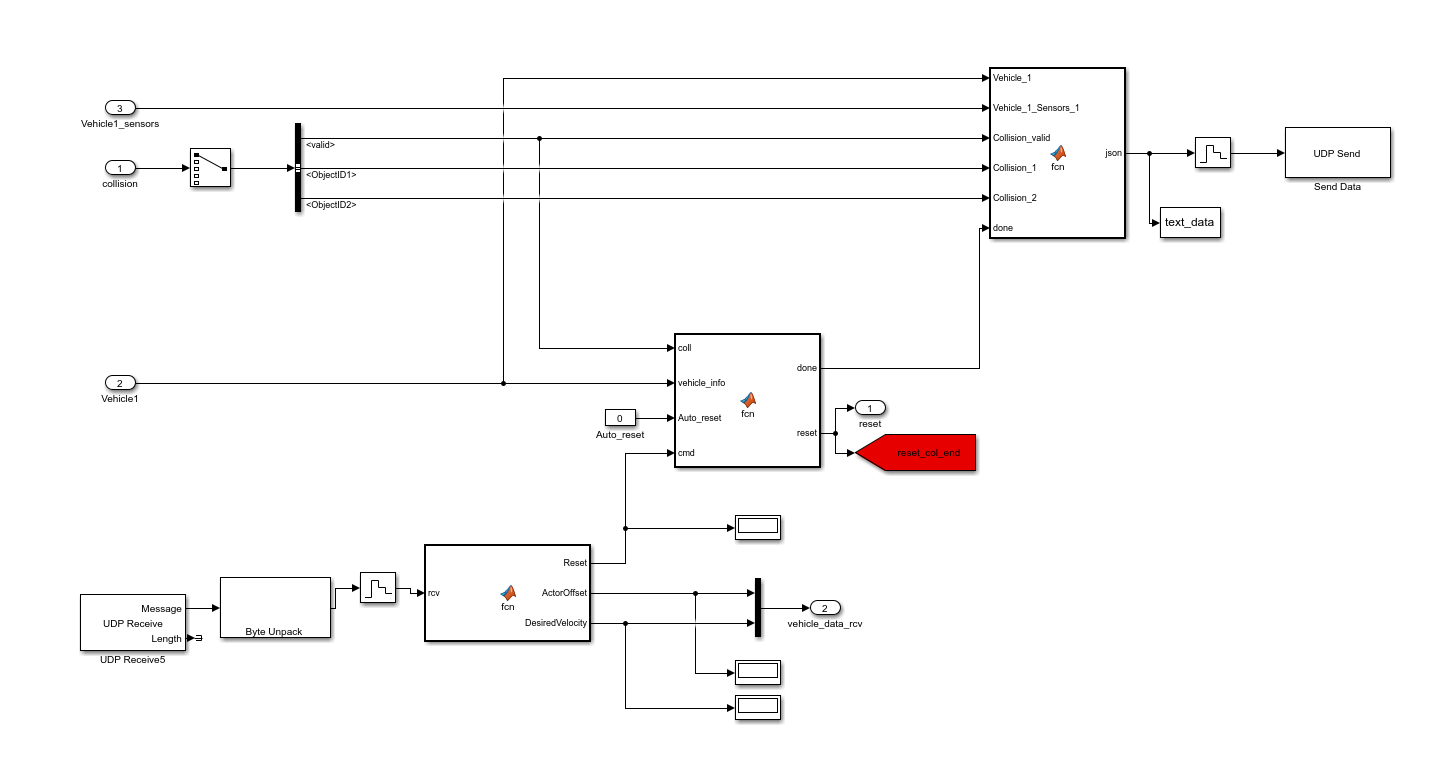
\includegraphics[width=0.95\linewidth]{Figures/simulink/inside-Environment}
	\caption{فایل سیمولینک - داخل بلوک \lr{Environment}}
	\label{fig:inside-environment}
\end{figure}

اگر به شکل 
\ref{fig:inside-environment}
دقت شود دو بلوک 
\lr{UDP}
دیده می‌شود. (بلوک 
\lr{UDP Send}
در بالا سمت راست و بلوک 
\lr{UDP Receive}
در پایین سمت چپ شکل 
\ref{fig:inside-environment}
)
این دو بلوک برای فرستادن داده های مورد نیاز به پایتون و گرفتن دستور های کنترلی از پایتون در سیمولینک تعبیه شده اند.

\begin{note}
	
اگر نمودار شکل
\ref{fig:block-diagram}
در نظر داشته باشیم، خواهیم یافت که این بلوک در شاخه پایینی ارتباط بین سیمولینک و پایتون قرارا دارد که از روش های شبکه کردن بین این دو انجام می‌شود. این بلوک صرفا داده‌های پویا را از متلب به سیمولینک انتقال می‌دهد و با داده‌های استاتیک کاری ندارد. 

\end{note}

 در جدول
\ref{tab:Reciver-Send}
 اطلاعات دقیق شبکه برای این دو بلوک دیده می‌شود. گفتنی است که این داده ها به نحوه مناسب کد شده‌اند تا تنها با استفاده از این دو بلوک بتوان داده ها را منتقل کرد.


\begin{table}
\tableset{
	\begin{tabular}{|c|c|c|c|c|}
		\hline\rowcolor{lightgray}
		نام بلوک & نوع بلوک & \lr{IP} & \lr{Port} & توضیحات
		\\\hline\hline
		\lr{UDP Receiver} & گیرنده & \lr{localhost} & 8070 &
		\\\hline
		\lr{Send Data} & فرستنده & \lr{localhost} & 8031 &
		\\\hline
	\end{tabular}}
	\caption{اطلاعات بلوک های فرستندگی گیرندگی در سیمولینک}
	\label{tab:Reciver-Send}
\end{table}


روش کد شدن
\LTRfootnote{Encoding}
قبل از ارسال و یا دریافت در این دو بلوک کاملا با یکدیگر متفاوت هستند. این کار توسط بلوک‌های قبل و بعد دو بلوک مذکور انجام می‌شود. 



در شکل 
\ref{fig:inside-environment}
سه بلوک تابع متلب 
\LTRfootnote{Matlab-function block}
   وجود دارد که از مهم‌ترین نقش را دارند. این نقش‌ها در ادامه توضیح توضیح مفصل داده شده‌اند.
   
   خلاصه این وظایف در زیر آمده است:
   
   \begin{itemize}
   		\item \textbf{بلوک فرستنده} :
   		این بلوک در سمت بالا سمت راست تمام اطلاعاتی که به بلوک کلی 
   		\lr{Environment}
   		وارد می‌شود را به نحوی مناسب به همراه متغیر \texttt{done} که از یک تابع متلب دیگر خارج می‌شود را برای پایتون طی ساختار مشخصی (جیسون) ارسال می‌کند. موضوع به صورت بسیط در بخش
   		\ref{ch:fani|sec:simulink|sub:json}
   		مورد بررسی قرار گرفته است.
   		\item \textbf{بلوک گیرنده} :
   		این بلوک تنها وظیفه آن این است که داده هایی که پس از بلوک \lr{Byte Unpacking} آمده است ، را انتخاب می‌کند که هر یک از این دیتا ها چه مفهومی هستند. از آن‌جا که ۳ داده کنترلی (لاین و سرعت و ریست) از طرف پایتون ارسال می‌شود، بلوک \lr{Byte Unpacking} وظیفه این ۳ داده را به فرمت \texttt{double} در می‌آورد (این فرمت در سمت پایتون نیز به همین شکل قرار داد شده‌است). بنابراین این بلوک \lr{Byte Unpacking} است که کار اصلی را انجام می‌دهد و تنها وظیفه این بلوک تفکیک و اسم گذاری بر‌روی خروجی بلوک \lr{Byte Unpacking} است.
   
   		\item \textbf{بلوک محاسبه تمام شدن و ریست کردن} :
   		این بلوک با دو خروجی مهم می‌دهد. یکی از آن خروجی ها \texttt{done} است که توسط بلوک فرستنده نیز برای پایتون ارسال می‌شود. و مقدار دیگری را که خروجی می‌دهد دستور ریست کردن است. این دستور در لبه مثبت (از صفر به یک برسد) ریست می‌کند. منطق این بلوک یک منطق باینری است که در شکل 
   		\ref{fig:done-reset-logical}
   		روش محاسبه آن نیز آمده است. 
   		همچنین این بلوک یک مقدار به اسم \texttt{Auto\_reset\_flag} نیز به عنوان ورودی دریافت می‌کند. این مقدار که می‌تواند صفر و یا یک باشد، تصمیم می‌گیرد که در صورتی که \LRE{\texttt{done = 1}} شد آیا ریست کند و یا ریست نکند. اگر یک باشد ریست می‌کند وگرنه منتظر رسیدن دستور از پایتون می‌ماند.
   		
   \end{itemize}

\begin{figure}
	\centering
	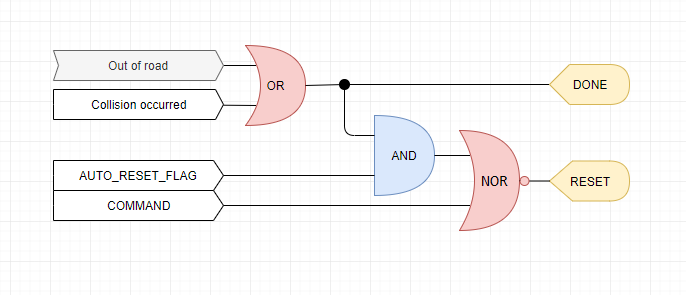
\includegraphics[width=0.7\linewidth]{Figures/done-reset-logical}
	\caption{منطق محاسبه تمام شدن و دستور ریست کردن}
	\label{fig:done-reset-logical}
\end{figure}

   
\subsection{بررسی ساختار داده های ارسالی  و کد آن در سیمولینک}\label{ch:fani|sec:simulink|sub:json}
   
   بلوک فرستنده در شکل
   \ref{fig:inside-environment}
   اطلاعات دریافت شده را طی ساختار مشخصی به ساختار جیسون در می‌آورد.
   نمونه ای از این ساختار در شکل
   \ref{fig:block-diagram}
    آمده است.
%\begin{figure}
%	\centering
%	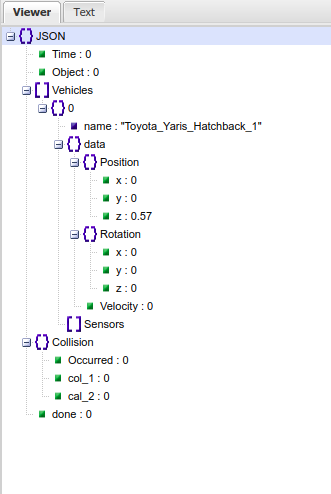
\includegraphics[height=8cm]{Figures/simulink/json-env}
%	\caption{}
%	\label{fig:json-env}
%	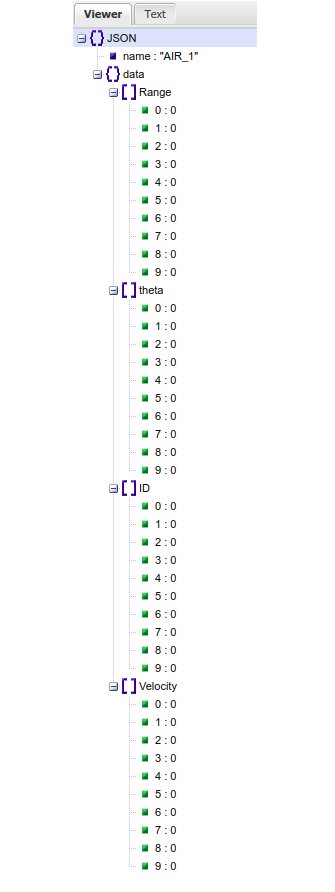
\includegraphics[height=8cm]{Figures/simulink/json-sensor}
%	\caption{}
%	\label{fig:json-sensor}
%	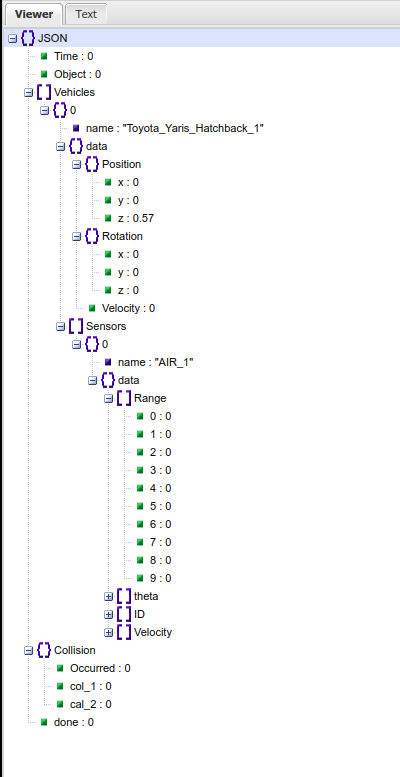
\includegraphics[height=8cm]{Figures/simulink/json-total}
%	\caption{}
%	\label{fig:json-total}
%\end{figure}
   
   
   
%\begin{latin}
%\begin{lstlisting}[language=json]
%'{"Time":0,"Object":0,"Vehicles":[{"name":"Toyota_Yaris_Hatchback_1","data":{"Position":{"x":0.00000e+00,"y":0.00000e+00,"z":5.70000e-01},"Rotation":{"x":0.00000e+00,"y":0.00000e+00,"z":0.00000e+00},"Velocity":0.00000e+00},"Sensors":[{"name":"AIR_1","data":{"Range":[0.00000e+00,0.00000e+00,0.00000e+00,0.00000e+00,0.00000e+00,0.00000e+00,0.00000e+00,0.00000e+00,0.00000e+00,0.00000e+00],"theta":[0.00000e+00,0.00000e+00,0.00000e+00,0.00000e+00,0.00000e+00,0.00000e+00,0.00000e+00,0.00000e+00,0.00000e+00,0.00000e+00],"ID":[0.00000e+00,0.00000e+00,0.00000e+00,0.00000e+00,0.00000e+00,0.00000e+00,0.00000e+00,0.00000e+00,0.00000e+00,0.00000e+00],"Velocity":[0.00000e+00,0.00000e+00,0.00000e+00,0.00000e+00,0.00000e+00,0.00000e+00,0.00000e+00,0.00000e+00,0.00000e+00,0.00000e+00]}}]}],"Collision":{"Occurred":0,"col_1": 0,"cal_2": 0},"done":0}'
%\end{lstlisting}
%\end{latin}
   
  
   
   
   

\begin{figure}[h!]
  	\centering
  	\subfigure[اطلاعات خام جیسون کلی]{%
  		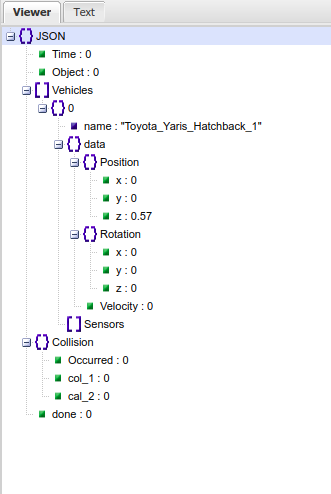
\includegraphics[height=8cm]{Figures/simulink/json-env}
   		\label{subfig:json-env}
  	}
%  	\hspace*{1.5cm} % space between two figures
  	\subfigure[جیسون سنسور]{%
  		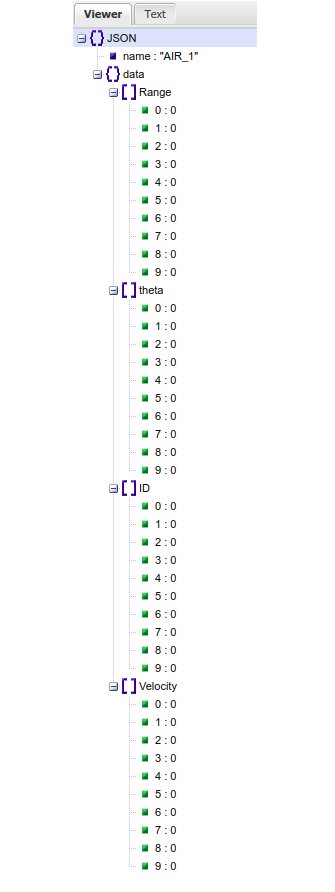
\includegraphics[height=8cm]{Figures/simulink/json-sensor}
   		\label{subfig:json-sensor}
  	}
%  	\\ % place in new line
%  	\hspace*{1.5cm} % space between two figures
  	\subfigure[شکل ادغام شده ]{%
  		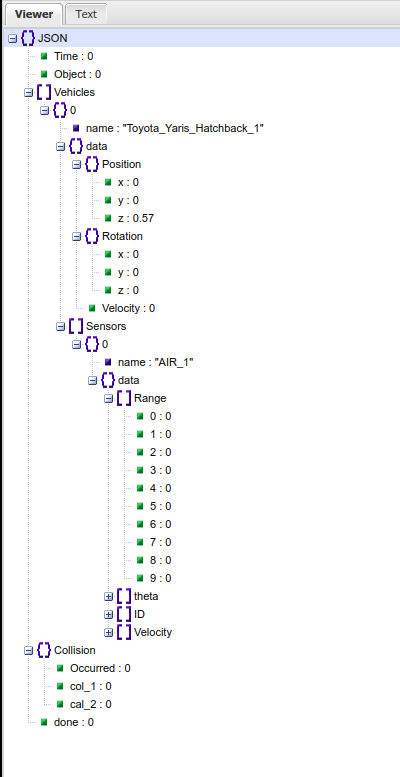
\includegraphics[height=8cm]{Figures/simulink/json-total}
   		\label{subfig:json-total}
  	}
  	\caption[ساختار جیسون برای بلوک های سیمولینک]{%
  		تصویر
  	\subref{subfig:json-env}
  	نحوه ساختار‌دهی کلی در بلوک تابع متلب واقع در زیرسیستم 
	\lr{Environment}
	را نشان می‌دهد. در این قسمت اطلاعات ماشین شامل دو قسمت \lr{data} و \lr{Sensors} است. اطلاعات سنسور های این ماشین  از تصویر \subref{subfig:json-sensor} تامین می‌شود. این ساختار در همان زیرسیستم ماشین تبدیل به جیسون شده و برای زیر‌سیستم \lr{Environmnet} ارسال می‌شود. قسمت سنسور یک آرایه است تا بتوان چندین سنسور مختلف را برای آن ارسال کرد. بنابراین ساختاری مانند تصویر \subref{subfig:json-total} باید را در نهایت برای پایتون ارسال می‌کند.
	\footnotemark
  	}
  	\label{fig:json-total}
\end{figure}
	\RTLfootnotetext{این عکس با استفاده از سایت
		\lr{\href{http://jsonviewer.stack.hu/}{http://jsonviewer.stack.hu/}}
	تهیه شده است.}
شکل \ref{subfig:json-sensor} همان ساختاری است که پیشتر در مورد آن صحبت شد. با توجه به این که این ساختار (در ادامه خواهید دید که) در اطلاعات سنسور ماشین به کار گرفته می‌شود و هر سنسور ممکن است اطلاعات خاص خود را داشته باشد. برای یکسان‌سازی این اطلاعات، در اولین لایه دو گزینه \lr{data} و \lr{name} را به طور قرار دادی بین همه سنسور ها یکسان است تا در کد پایتون بتوان با توجه به اسم آن ها ادامه ساختار که در \lr{data} می‌باشد، قابل تشخیص باشد. اما از آن‌جا که صرفا از اطلاعات یک سنسور استفاده شده است این شکل ساختار‌دهی تنها یک گزینه برای توسعه های آتی آن است.

در این ساختار ۴ اطلاعات نشان داده شده که هر یک از آن اطلاعات خود یک بردار ۱۰ تایی است، برای پایتون ارسال می‌شود. 

شکل 
\ref{subfig:json-env}
ساختار کلی است که محیط \lr{Environmnet} از آن استفاده می‌کند. در این بلوک علاوه بر داده هایی مانند اطلاعات ماشین و سنسورش، اطلاعات تصادف و اطلاعات تمام شدن و یا نشدن شبیه سازی که پیش‌‌تر در مورد آن اطلاعات صحبت شد، دو اطلاعات اضافه دیگر نیز می‌فرستد.
\begin{itemize}
	\item \texttt{Time} :
	زمان شبیه سازی را همراه با دیتا دیگر ارسال می‌کند و به اصلاح یک ساختار زمانی ایجاد می‌شود.
	\LTRfootnote{Time-struct}
	\item \texttt{Object} :
	این عبارت کمک به کد پایتون می‌کند که ماشین هدف و یا عامل را از بین ماشین های موجود در لیست \texttt{Vehicles} بیابد. 
	\RTLfootnote{از آنجایی که در این پروژه  لیست \lr{Vehicles} یک آبجکت بیشتر ندارد، پس این بخش نیز صرفا ظرفیت توسعه‌پذیری این کد را بالا می‌برد.}
\end{itemize}

در نهایت با ادغام شدن اطلاعات سنسور نیز، ساختار کلی به شکل \ref{subfig:json-total} در خواهد آمد . در بخش
\ref{ch:fani|sec:chalenges}
از برخی از چالش های ساختاردهی کردن به این شکل، صحبت خواهد شد. همچنین خروجی نهایی آن نیز را می‌توانید در 
\hyperref[code:json]{همان بخش}
 بیابید.

\section{بررسی جزییات بخش پایتون}\label{ch:fani|sec:python}
بارها اشاره شد که پایتون بخش اصل تصمیم‌گیری را برعهده دارد. در بخش 
\ref{ch:fani|sec:simulink}
سعی شد تا به نحو مناسبی دیتای محیط شبیه‌سازی را به پایتون منتقل کند و دستورات کنترلی را نیز از پایتون به محیط شبیه‌سازی ارسال کند. در این بخش بر روی مفاهیم پایتونی آن مانور می‌دهیم.

از آن‌جا که کد پایتون باید به سیمولینک متصل شود و دیتا را به الگوریتم کنترلی خود (که از الگوریتم های یادگیری تقویتی استفاده شده است) ، برساند و از آن جا دستورات را دریافت کتد و به سیمولینک برساند، نیازمند لایه هایی است که هر لایه بخشی از این کار ها انجام دهد.

\subsection{معرفی لایه های کد پایتون}\label{ch:fani|sec:python|sub:layers}
کد پایتون از لایه های مختلف تشکیل شده است. از هر لایه به لایه بعدی سطح زبان بالاتر می‌رود. این لایه ها در شکل 
\ref{ch:fani|sec:python|sub:layers}
مشخص شده اند. در لایه های ابتدایی، سطح استفاده از دستورات بسیار ابتدایی است و در هر لایه با تعریف توابع و کلاس هایی این امکان را ایجاد کرده اند که بدون در نظر گرفتن این که در سطوح پایین‌تر چه اتفاقاتی می‌افتد، در سطوح بالاتر از آن امکانات استفاده کرد. در ادامه این بحث مفصل توضیح داده خواهد شد.



\begin{figure}
	\centering
	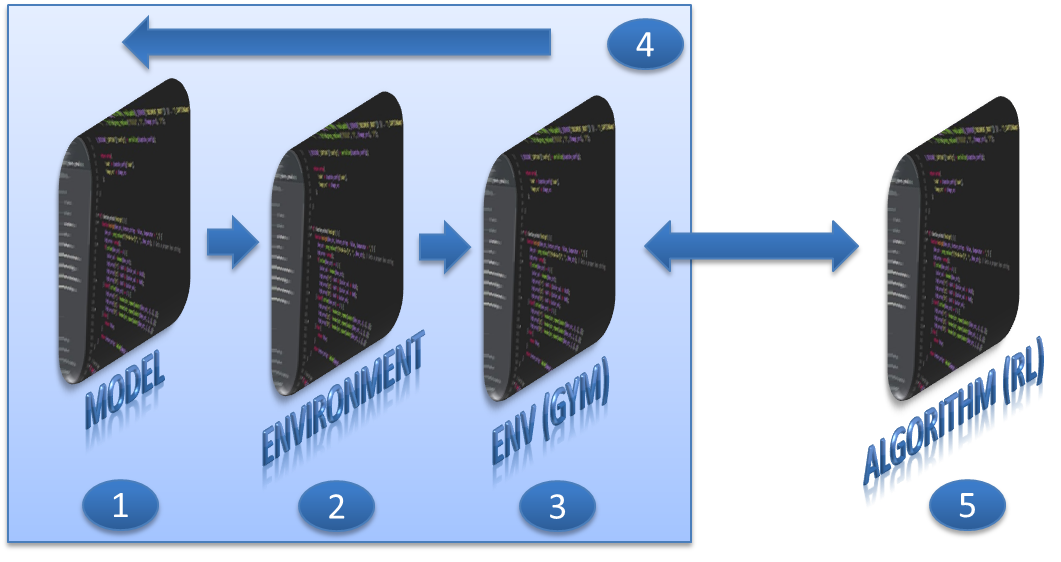
\includegraphics[width=0.8\linewidth]{Figures/python-layers-white}
	\caption{بلوک دیالگرام لایه های پایتون}
	\label{fig:python-layers}
\end{figure}
در شکل 
\ref{fig:python-layers}
۴ لایه برنامه نویسی شده با ۵ عدد نشان داده شده است. توضیحات زیر متناسب با هر‌یک از این شماره ها در نظر گرفته شده اند:




\begin{circlelist}
	\item \textbf{\lr{Model}} :
	در این لایه، با استفاده از موتور متلب با متلب و سیمولینک ارتباط برقرار می‌کند و با این ارتباط دو وظیفه بسیار مهم را انجام می‌دهد. 
	\begin{alphabetlist}
		\item 
		ساخت مدل هایی مانند اتومبیل و جاده و دریافت اطلاعات ضروری آن ها در متلب
		\item 
		تعریف کلاس \lr{sim} و ارسال دستوراتی مانند شروع کردن، توقف کردن، مکث کردن، ادامه دادن و ... به سیمولینک.
	\end{alphabetlist}
این لایه صرفا از اطلاعات استاتیک سیمولینک استفاده می‌کند.

	\item \textbf{\lr{Environment}} :
	این لایه برای ارتباط با زیرسیستم \lr{Environment} که پیشتر آن‌را در شکل 
	\ref{fig:simulink-env}
	مشاهده کردید، ساخته شده است. در این لایه با استفاده از ابزار هایی که لایه 
	\lr{Model}
	در اختیار آن قرار می‌دهد، به سادگی آبجکت هایی ماند ماشین و جاده را می‌سازد و با استفاده از اطلاعات شبکه که در جدول 
	\ref{tab:Reciver-Send}
	آمده است، با سیمولینک ارتباط برقرار می‌کند و آن اطلاعات پویا را دریافت می‌کند و دستورات کنترلی را برای آن ارسال می‌کند.
	
	این لایه از موتور متلب استفاده نمی‌کند بلکه از روش های شبکه ای استفاده می‌کند. 
	\item \textbf{\lr{Env}} :
	این لایه یک آبجکت از کلاس 
	\lr{Environment}
	را دریافت می‌کند و تمامی نیاز های خود را در مورد هر مسیله‌ای که به ارتباط با محیط متلب و یا سیمولینک به آن واگذار می‌کند و تمرکز آن برروی مفاهیم یادگیری تقویتی مانند 
	 \begin{enuminline}
	 	\item فضای مشاهده
	 	\LTRfootnote{Observation space}
	 	\item فضای حرکت
	 	\LTRfootnote{Action space}
	 	\item  تعریف حرکت
		\item تعریف حالت 
		\item تعریف امتیاز
 	\end{enuminline} 
 و ... می‌باشد.
 
	
	\item \textbf{\lr{gym}} :
	در نهایت یک مجموعه داریم که هر یک وظایف مربوط به خود را دارند. در این قسمت کد ما که در لایه \lr{Env} به \lr{gym} نزدیک شده است، با فراخوانی لایه های پیشین به ترتیب از بالا به پایین (از نظر سطح) فراخوانی می‌شود و در هر لایه آبجکت‌هایی از کلاس‌های موجود در لایه پایین تر فراخوانی می‌شود. از این رو جهت پیکان بر عکس است. 
	
	در مورد \lr{gym} در فصل 
	\ref{ch:openai-gym}
	به صورت مفصل بحث شده‌است.
	
	\item \textbf{\lr{Algorithm}} :
	در لایه های پیشین سینتکس کد \lr{gym} ایجاد شده است و این لایه بر توسعه الگوریتم های یادگیری تقویتی که در فصل 
	\ref{ch:RL}
	مورد بررسی مفصل قرار گرفته است، تمرکز دارد.
	
	می‌توان گفت این لایه نقش رییس و یا مغز کار را دارد و باقی لایه ها کارگرانی هستند که وظیفه دارند که اطلاعات را به شکلی مناسب این لایه، برای آن منتقل کنند.
\end{circlelist}	


\section{بررسی دقیق تر برخی چالش های فنی پروژه}\label{ch:fani|sec:chalenges}



\code[json,label={code:json}]{structure-string.json}

   








%\thispagestyle{empty}
%
%\section{مقدمه}
%
%فصل مقدمه یک پایان نامه، با بیان نیاز موضوع، تعريف مسئله و اهمیت آن در یک یا چند بند (پاراگراف) آغاز مي‌شود\footnote{شروع مقدمه نبايد چنان طولاني باشد كه هدف اصلي را تحت‌ تاثير قرار دهد.}  و با مرور پيشينه موضوع (سابقه کارهای انجام‌شده پیشین که ارتباط مستقیمی با مسئله مورد بررسی دارند) ادامه مي‌يابد. سپس در یک یا دو بند توضیح داده مي‌شود كه در این پایان نامه، چه ديدگاه يا راهكار جدیدي نسبت به مسئله (موضوع) مورد بررسي وجود دارد. به‌عبارت دیگر نوآوری‌ها به‌صورت کاملاً شفاف و صریح بیان می‌شود. در ادامه ممکن است به نتايج بدست‌آمده نیز به‌طور مختصر و کلی اشاره ‌شود. در آخرین بند از مقدمه به محتواي فصل‌هاي بعدي پایان نامه به‌اختصار اشاره مي‌شود.\\
%برای مشاهده دستورالعمل کامل دانشگاه صنعتی امیرکبیر(پلی تکنیک تهران) به \cite{zakeri} یا به سایت
%%
%\href{http://library.aut.ac.ir/Thesis%20Guide}{کتابخانه دانشگاه صنعتی امیرکبیر(پلی تکنیک تهران)}%
%مراجعه نمایید.
%
%نگارش صحيح يک پایان نامه در فهم آسان آن بسيار موثر است. در اين فصل مهمترین قواعد نگارشی که باید مورد توجه جدی نگارنده قرار گیرد، به اختصار بیان می‌شود. اين قواعد را مي‌توان در محورهای اصلی زير دسته‌بندی کرد:
%\begin{itemize}
%\item
%فارسی نویسی
%\item
%رعایت املای صحيح 
%\item
%رعایت قواعد نشانه‌گذاری
%\end{itemize}
%\section{فارسی نویسی}
%در حد امکان سعی کنيد به جاي کلمات غير‌فارسی از معادل فارسی آنها استفاده کنيد، به‌ويژه در مواردی که معادل فارسی مصطلح و رايج است‌.‌ به‌طور مثال استفاده از کلمه «لذا» به‌جای «برای همين» يا «به‌همين دليل» توجيهی ندارد‌. همچنين کلمه «پردازش» زيباتر از «پروسس» و معادل فارسی «ريز‌پردازنده» مناسب‌تر از «ميکروپروسسور» است‌.‌ در اين‌گونه موارد چنانچه احتمال عدم آشنايی خواننده با معادل فارسی وجود دارد، يا اصطلاح غير‌فارسی معمول‌تر است، در اولين ظهور کلمه فارسی، اصل غير‌فارسی آن به‌صورت پاورقي آورده شود‌.‌ اگر به‌ناچار بايد کلمات انگليسی در لابه‌لای جملات گنجانده شوند، از هر طرف يک فاصله بين آنها و کلمات فارسی پیش و پس از آنها در‌نظر گرفته شود‌.‌ چنانچه در پایان نامه از مختصر‌نويسی استفاده شود، لازم است در اولين استفاده، تفصيل آن در پاورقي آورده شود‌.‌ 
%
%\section{رعایت املای صحيح }
%رعايت املاي صحيح فارسي به مطالعه و درک راحت‌تر کمک مي‌کند. همچنين در نوشته‌هاي فارسي بايد در حد امکان از همزه « ء، أ، ؤ، ة، إ، ئ» استفاده نشود‌.‌ به‌عنوان مثال «اجزاء هواپیما» و «آئين نگارش» ناصحیح، اما «اجزاي هواپیما» و «آيين نگارش» صحيح هستند.‌
%\section{رعایت قواعد نشانه‌گذاری}
%منظور از نشانه‌گذاري به‌کار‌بردن علامت‌ها و نشانه‌هايي است که خواندن و فهم درست یک جمله را ممکن و آسان مي‌کند. در ادامه نشانه‌هاي معمول و متداول در زبان فارسي و موارد کاربرد آنها به اختصار معرفی می‌شوند.
%
%\subsection{ويرگول}
%ويرگول نشانه ضرورت یک مکث کوتاه است و در موارد زير به‌کار مي‌رود:
%\begin{itemize}
%\item
%در ميان دو کلمه که احتمال داده شود خواننده آنها را با کسره اضافه بخواند، يا نبودن ويرگول موجب بروز اشتباه در خواندن جمله شود.
%\item
%در موردي که کلمه يا عبارتي به‌‌‌‌عنوان توضيح، در ضمن یک جمله آورده شود. مثلاً برای کنترل وضعیت فضاپیماها، به‌دلیل آن‌که در خارج از جو هستند، نمی‌توان از بالک‌های آیرودینامیکی استفاده کرد.
%\item
%جدا‌کردن بخش‌هاي مختلف يک نشاني يا یک مرجع
%\item
%موارد دیگر از این قبیل
%\end{itemize}
%پیش از ويرگول نبايد فاصله گذاشته شود و پس از آن يک فاصله لازم است و بيشتر از آن صحیح نیست.
%\subsection{نقطه}
%نقطه نشانه پایان یک جمله است. پیش از نقطه نبايد فاصله گذاشته شود و پس از آن يک فاصله لازم است و بيشتر از آن صحیح نیست.
%\subsection{دونقطه}
%موارد کاربرد دونقطه عبارتند از:
%\begin{itemize}
%\item
%پيش از نقل قول مستقيم
%\item
%پيش از بيان تفصيل مطلبي که به اجمال به آن اشاره شده‌است.
%\item
%پس از واژه‌اي که معني آن در برابرش آورده و نوشته مي‌شود.
%\item
%پس از کلمات تفسير‌کننده از قبيل «يعني» و ...
%\end{itemize}
%پیش از دونقطه نبايد فاصله گذاشته شود و پس از آن يک فاصله لازم است و بيشتر از آن صحیح نیست.
%\subsection{گیومه}
%موارد کاربرد گیومه عبارتند از:
%\begin{itemize}
%\item
%وقتي که عين گفته يا نوشته کسي را در ضمن نوشته و مطلب خود مي‌آوريم. 
%\item
%در آغاز و پايان کلمات و اصطلاحات علمي و يا هر کلمه و عبارتي که بايد به‌صورت ممتاز از قسمت‌هاي ديگر نشان داده شود.
%\item
%در ذکر عنوان مقاله‌ها، رساله‌ها، اشعار، روزنامه‌ها و ...
%\end{itemize}
%\subsection{نشانه پرسشی}
%پیش از «؟» نبايد فاصله گذاشته شود و پس از آن يک فاصله لازم است و بيشتر از آن صحیح نیست.
%\subsection{خط تیره}
%موارد کاربرد خط تیره عبارتند از:
%\begin{itemize}
%\item
%جدا‌کردن عبارت‌هاي توضيحي، بدل، عطف بيان و ...
%\item
%به‌جاي حرف اضافه «تا» و «به» بين تاريخ‌ها، اعداد و کلمات
%\end{itemize}
%\subsection{پرانتز}
%موارد کاربرد پرانتز عبارتند از:
%\begin{itemize}
%\item
%به‌معني «يا» و «يعني» و وقتي که یک کلمه يا عبارت را براي توضيح بيشتر کلام بياورند.
%\item
%وقتي که نويسنده بخواهد آگاهي‌هاي بيشتر (اطلاعات تکميلي) به خواننده عرضه کند.
%\item
%براي ذکر مرجع در پايان مثال‌ها و شواهد.
%\end{itemize}
%نکته: بین کلمه یا عبارت داخل پرانتز و پرانتز باز و بسته نباید فاصله وجود داشته باشد.
%\section{جدا یا سرهم نوشتن برخی کلمات}
%تقريباً تمامي کلمات مرکب در زبان فارسي بايد از هم جدا نوشته شوند؛ به استثناي صفات فاعلي مانند «عملگر»، «باغبان» و يا «دانشمند» و کلماتي نظير «اينکه»، «آنها». در ادامه به نمونه‌هايي از مواردي که بايد اجزاي يک کلمه جدا، اما بدون فاصله نوشته شوند، اشاره مي‌شود‌:
%\begin{enumerate}
%\item
%در افعال مضارع و ماضی استمراری که با «می» شروع می‌شوند، لازم است که در عين جدا نوشتن، «می» از بخش بعدي فعل جدا نيافتد‌.‌ برای اين منظور بايد از «فاصله متصل» استفاده و «می» در اول فعل با \lr{SS}\LTRfootnote{Shift+Ctrl+@} از آن جدا شود.‌ به‌طور مثال «می‌شود» به‌جاي «می شود». 
%\item
%	«ها»ی جمع بايد از کلمه جمع بسته‌شده جدا نوشته شود؛ مگر در برخی کلمات مانند «آنها». اين امر در مورد کلمات غير‌فارسي که وارد زبان فارسي شده‌اند و با حرف «ها» جمع بسته می‌شوند، مانند «کانال‌ها» يا «فرمول‌ها» مورد تاکيد است.
%\item
%	حروف اضافه مانند «به» وقتي به‌صورت ترکيب ثابت همراه کلمه پس از خود آورده می‌شوند، بهتر است با \lr{SS} از آن جدا شوند‌.‌ مانند «به‌صورت»، «به‌عنوان» و «به‌‌‌لحاظ»‌.‌ لازم به ذکر است هنگامی که حرف اضافه «به» با کلمه پس از خود معناي قيدي داشته باشد، مثل «بشدت» يا «بسادگي»، بهتر است که به‌صورت چسبيده نوشته شود‌.
%\item
%	کلمات فارسی نبايد با قواعد عربی جمع بسته شوند؛ پس «پيشنهادها» صحيح و «پيشنهادات» اشتباه است‌.‌
%\item
%	اسم‌ها و صفت‌هاي دو‌قسمتي مثل «خط‌چين» و «نوشته‌شده» با \lr{SS} از هم جدا می‌شود‌.‌
%\item
%	شناسه‌ها با \lr{SS} از کلمه اصلي جدا می‌شود‌.‌ مثل «شده‌اند»‌ و «شده‌است». 
%\item
%	‌ «است» هنگامی که نقش شناسه را داشته باشد توسط \lr{SS} از قسمت اصلي جدا می‌شود‌.‌ مانند «گفته‌است»‌.
%\item
%	بند پیشین نبايد باعث افراط در استفاده از فاصله متصل شود. مثلاً عبارت «نوشته می‌شود‌« صحيح و عبارت «نوشته‌می‌شود» ناصحیح است. 
%\item
%	فعل‌هاي دو‌کلمه‌اي که معناي اجزاي آنها کاملاً با معناي کل متفاوت است، بهتر است که با \lr{SS} از هم جدا ‌شوند‌.‌
%\item
%	کلمات مرکب مثل کلمه «دوکلمه‌اي» در عبارت «فعل‌هاي دوکلمه‌اي» و «يادداشت‌برداري».
%\item
%	مصدرهاي دو قسمتي با \lr{SS} از هم جدا می‌شوند‌.‌ مثل «ذوب‌کردن» و «واردکردن»‌.
%\item
%	 صفات تفضيلي مثل « آسان‌تر».
%\end{enumerate}
%

\chapter{مشخصات یک پایان نامه و گزارش علمی}

اگرچه براي همه انواع نوشته‌ها، مشخصات و ويژگي‌هاي واحد و معيني نمي‌توان ذكر كرد، با اين حال در یک پایان نامه یا گزارش علمی باید نکات و موارد کلی که در این فصل ذکر می‌شود، بطور کامل رعایت شده باشد. 

دقت كنيد كه پس از عنوان فصل بايد حداقل توضیحی کوتاه در مورد موضوع نوشته شود و نمي‌توان مستقيماً بعد از آن عنوان بخش را نوشت و همين طور پس از عناوين بخش‌ها و زيربخش‌ها.(مانند دستورالعمل حاضر)
\section{برخورداری از غنای علمی }

يك پایان نامه بايد پیش از هر چيز به‌لحاظ علمي از غناي لازم برخوردار باشد. يعني هدف و پيام روشني داشته باشد و از پيش‌زمينه علمي، بيان دلايل علمی، ارجاعات مورد نیاز و نتيجه‌گيري شفاف بهره ببرد. 

\section{ارجاع به‌موقع و صحیح به منابع دیگر}
هر جمله‌ای که در یک پایان نامه نوشته می‌شود یا یک جمله کاملاً بدیهی است یا باید دلیل آن بیان شود و یا اینکه باید به منبعی که آن موضوع را نقل یا اثبات کرده، ارجاع داده شود. اگر مطلب يا گفتاري از منبعی عيناً در گزارش نقل مي‌شود، بايد آن مطلب داخل گيومه قرار گيرد و با ذكر ماخذ و شماره صفحه، به آن اشاره گردد.


\section{ساده‌نویسی }
سادگی از ضروريات يك نوشته است. نويسنده بايد ساده، روان و در عين حال شيوا و رسا بنويسد و عبارات مبهم، جملات پيچيده و كلمات نامأنوس در نوشته خود به‌كار نبرد. اگر چه افراط در اين امر نيز، به شيوايي نوشته صدمه مي‌زند. به‌كارگیری لغات و اصطلاحات دشوار و دور از ذهن و عبارات و جملات نامنظم و مبهم موجب ايجاد اشكال در فهم خواننده خواهد شد‌. 

 براي ساده‌نويسي بايد در حد امكان از به‌كارگيری كلمات «مي‌بايست»، «بايستي»، «گرديد»، «بوده باشد» و مانند آنها كه تكلف‌آور، غلط مصطلح و يا غيرشيوا هستند، به‌جای «بايد»، «است»، «شد» و مثل آنها، اجتناب شود‌.‌ همين‌طور، «در‌جهت» نمی‌تواند جايگزين خوبی برای كلمه روانی مثل «برای» باشد‌. ‌كلمات و جملات روان و ساده مي‌توانند اغلب مفاهيم را براحتی منتقل كنند‌.‌
 
دقت در تنظیم بندها (پاراگراف‌ها) نيز كمك شاياني به روانی و سادگی فهم مطلب مي‌كند‌.‌ بندهای طولانی نيز مانند جملات طولانی مي‌توانند خسته‌كننده باشند و خواننده را سردرگم كنند‌.‌ يك بند نبايد کمتر از سه یا چهار سطر یا بيشتر از $10$ تا 15 سطر باشد.‌ 

\section{وحدت موضوع}

نویسنده بايد در سراسر نوشته از اصل موضوع دور نيافتد و تمام بحث‌ها، مثال‌ها و اجزاي نوشته با هماهنگي كامل، پيرامون موضوع اصلي باشد و تاثيري واحد در ذهن خواننده القا كند. 
\section{اختصار}

پایان نامه یا گزارش علمی بايد در حد امكان، مختصر و مفيد باشد و از بحث‌هاي غير ضروري در آن پرهيز شود. نوشتن مطالب ارزشمندي كه هيچ ربطي به موضوع ندارد، فاقد ارزش علمي است.
\section{رعایت نكات دستوري و نشانه‌گذاري}
در سراسر پایان نامه بايد قواعد دستوري رعايت شود و اركان و اجزاي جمله در جاي مناسب خود آورده شود. همچنین رعايت قواعد نشانه‌گذاري سبب مي‌شود كه بيان نويسنده روشن باشد و خواننده به سهولت و با کمترین صرف انرژی مطالب را مطالعه و درك كند.
\section{توجه به معلومات ذهنی مخاطب}
نويسنده بايد همواره مخاطب خود را در برابر خود تصور كند و با توجه به معلومات ذهني مخاطب  تمامي پیش‌نیازهای لازم براي درك مطالب مورد بحث را، از پیش براي مخاطب فراهم كند.

\section{رعایت مراحل اصولی نگارش}
هر کار علمی زمانی به بهترین شکل قابل انجام است که بر اساس یک برنامه‌ریزی مشخص انجام شود. تهیه یک متن علمي با کیفیت نیز نیازمند برنامه‌ریزی مناسب و اجرای منظم آن می‌باشد. مراحل نگارش را عموماً می‌توان به ترتیب زیر درنظر گرفت:
\begin{itemize}


\item	تهيه فهرستی از عناوین اصلي و فرعی که باید نوشته شود
\item 	اولویت‌بندی و تعیین ترتیب منطقی فصل‌ها و بخش‌های گزارش
\item 	گردآوري اطلاعات اولیه راجع به هر بخش و زیربخش
\item 	تدوین مطالب جدیدی که باید به قلم نگارنده به گزارش اضافه شود
\item 	تایپ كردن مطالب با رعایت کامل نکاتی که در این دستورالعمل آموزش داده می‌شود
\end{itemize}
رعایت نظم و ترتیب در اجرای مراحل ذکر شده هم فرآیند تهیه پایان نامه یا گزارش علمی را برای نگارنده آسان می‌کند و هم کیفیت نگارش را به میزان قابل توجهی افزایش می‌دهد.

















\chapter{جمع‌بندي و نتيجه‌گيري و پیشنهادات}
%%%%%%%%%%%%%%%%%%%%%%%%%%%%%%%%%%%%%%%%%%%
در پايان گزارش‌هاي علمي و فني لازم است كه جمع‌بندي يا نتيجه‌گيري نهايي ارائه شود. در اين موارد مي‌توان آخرين فصل پایان نامه كه پیش از مراجع قرار مي‌گيرد را به اين امر اختصاص داد.
\section{پیشنهادات}
در این بخش پیشنهاداتی که محقق جهت ادامه تحقیقات دارد ارایه می‌گردد. دقت شود که پیشنهادات باید از  تحقیق انجام شده و نتایج ان حاصل شده باشد و از ذکر جملات کلی باید پرهیز کرد.

%--------------------------------------------------------------------------appendix( مراجع و پیوست ها)
\chapterfont{\vspace*{-2em}\centering\LARGE}%

\appendix
\bibliographystyle{plain-fa}
\bibliography{references}
\chapter*{‌پیوست}
\markboth{پیوست}{}
\addcontentsline{toc}{chapter}{پیوست}
موضوعات مرتبط با متن گزارش پایان نامه كه در يكی از گروه‌های زير قرار می‌گيرد، در بخش پيوست‌ها آورده شوند:
\begin{enumerate}
\item  اثبات های رياضی يا عمليات رياضی طولانی‌.‌
\item داده و اطلاعات نمونه (های) مورد مطالعه (\lr{Case Study}) چنانچه طولانی باشد‌.‌
\item نتايج كارهای ديگران چنانچه نياز به تفصيل باشد‌.‌
\item مجموعه تعاريف متغيرها و پارامترها، چنانچه طولانی بوده و در متن به انجام نرسيده باشد‌.‌
\end{enumerate}
% براي شماره‌گذاري روابط، جداول و اشكال موجود در پيوست‌ از ساختار متفاوتي نسبت به متن اصلي استفاده مي‌شود كه در زير به‌عنوان نمونه نمايش داده شده‌است. 
% \begin{equation}
%F=ma
%\end{equation}
\section*{کد میپل }
\begin{latin}
\begin{verbatim}

with(DifferentialGeometry):
with(Tensor):
DGsetup([x, y, z], M)
																	frame name: M
a := evalDG(D_x)
																	D_x
b := evalDG(-2 y z D_x+2 x D_y/z^3-D_z/z^2)


\end{verbatim}
\end{latin}
%--------------------------------------------------------------------------dictionary(واژه نامه ها)
%اگر مایل به داشتن صفحه واژه‌نامه نیستید، خط زیر را غیر فعال کنید.
\parindent=0pt
%
\chapter*{واژه‌نامه‌ی فارسی به انگلیسی}
\pagestyle{style9}

\addcontentsline{toc}{chapter}{واژه‌نامه‌ی فارسی به انگلیسی}
%%%%%%
\begin{multicols*}{2}

{\bf آ}
\vspace*{3mm}


\farsiTOenglish{اسکالر}{Scalar}


\vspace*{3mm}
{\bf ب}
\vspace*{3mm}

\farsiTOenglish{بالابر}{Lift}


\vspace*{3mm}
{\bf پ}
%%\vspace*{3mm}

\farsiTOenglish{پایا}{Invariant}



\vspace*{3mm}
{\bf ت}
%%\vspace*{3mm}

\farsiTOenglish{ تناظر }{Correspondence}


\vspace*{3mm}
{\bf ث}
%%\vspace*{3mm}

\farsiTOenglish{ثابت‌ساز}{Stabilizer}

\vspace*{3mm}
{\bf ج}
%%\vspace*{3mm}

\farsiTOenglish{جایگشت}{Permutation}



\vspace*{3mm}
{\bf چ}
%%\vspace*{3mm}


\farsiTOenglish{چند جمله‌ای }{Polynomial}

\vspace*{3mm}
{\bf ح}
%%\vspace*{3mm}

\farsiTOenglish{حاصل‌ضرب دکارتی}{Cartesian product}


\vspace*{3mm}
{\bf خ}
%%\vspace*{3mm}

\farsiTOenglish{خودریختی}{Automorphism}

\vspace*{3mm}
{\bf د}
%%\vspace*{3mm}

\farsiTOenglish{درجه}{Degree}


\vspace*{3mm}
{\bf ر}
%%\vspace*{3mm}


\farsiTOenglish{ریزپردازنده}{microprocessor}


\vspace*{3mm}
{\bf ز}
%%\vspace*{3mm}


\farsiTOenglish{زیرمدول}{Submodule}


\vspace*{3mm}
{\bf س}
%%\vspace*{3mm}

\farsiTOenglish{سرشت}{Character}


\vspace*{3mm}
{\bf ص}
%%\vspace*{3mm}

\farsiTOenglish{صادقانه}{Faithful}

\vspace*{3mm}
{\bf ض}
%%\vspace*{3mm}

\farsiTOenglish{ضرب داخلی}{Inner product}

\vspace*{3mm}
{\bf ط}
%%\vspace*{3mm}


\farsiTOenglish{طوقه}{Loop}


\vspace*{3mm}
{\bf ظ}
%%\vspace*{3mm}


\farsiTOenglish{ظرفیت}{Valency}
 
\vspace*{3mm}
{\bf ع}
%%\vspace*{3mm}


\farsiTOenglish{عدم مجاورت}{Nonadjacency}



\vspace*{3mm}
{\bf ف}
%%\vspace*{3mm}

\farsiTOenglish{فضای برداری}{Vector space}



\vspace*{3mm}
{\bf ک}
%%\vspace*{3mm}

\farsiTOenglish{کاملاً تحویل‌پذیر}{Complete reducibility}


\vspace*{3mm}
{\bf گ}
%%\vspace*{3mm}


\farsiTOenglish{گراف}{Graph}



\vspace*{3mm}
{\bf م}
%%\vspace*{3mm}

\farsiTOenglish{ماتریس جایگشتی}{Permutation matrix }


\vspace*{3mm}
{\bf ن}
%%\vspace*{3mm}

\farsiTOenglish{ناهمبند}{Disconnected}


\vspace*{3mm}
{\bf و}
%%\vspace*{3mm}

\farsiTOenglish{وارون‌پذیر}{Invertible}


\vspace*{3mm}
{\bf ه}
%%\vspace*{3mm}

\farsiTOenglish{همبند}{Connected}



\vspace*{3mm}
{\bf ی}
%%\vspace*{3mm}

\farsiTOenglish{یال}{Edge}




\end{multicols*}%
%%%%%%
\chapter*{ واژه‌نامه‌ی انگلیسی به فارسی}
\pagestyle{style9}
\lhead{\thepage}\rhead{واژه‌نامه‌ی انگلیسی به فارسی}
\addcontentsline{toc}{chapter}{واژه‌نامه‌ی انگلیسی به فارسی}

\LTRmulticolcolumns
\begin{multicols}{2}
{\hfill\bf  \lr{A}}
%%\vspace*{1.5mm}

\englishTOfarsi{Automorphism}{خودریختی}

\vspace*{3mm}
{\hfill\bf   \lr{B}}
%%\vspace*{1.5mm}

\englishTOfarsi{Bijection}{دوسویی}

\vspace*{3mm}
{\hfill\bf   \lr{C}}
%%\vspace*{1.5mm}

\englishTOfarsi{Cycle group}{گروه دوری}

\vspace*{3mm}
{\hfill\bf   \lr{D}}
%%\vspace*{1.5mm}

\englishTOfarsi{Degree}{درجه}

\vspace*{3mm}
{\hfill\bf   \lr{E}}
%%\vspace*{1.5mm}

\englishTOfarsi{Edge}{یال}

\vspace*{3mm}
{\hfill\bf   \lr{F}}
%%\vspace*{1.5mm}

\englishTOfarsi{Function}{تابع}

\vspace*{3mm}
{\hfill\bf   \lr{G}}
%%\vspace*{1.5mm}

\englishTOfarsi{Group}{گروه}

\vspace*{3mm}
{\hfill\bf   \lr{H}}
%%\vspace*{1.5mm}

\englishTOfarsi{Homomorphism}{همریختی}

\vspace*{3mm}
{\hfill\bf   \lr{I}}
%%\vspace*{1.5mm}

\englishTOfarsi{Invariant}{پایا}

\vspace*{3mm}
{\hfill\bf   \lr{L}}
%%\vspace*{1.5mm}

\englishTOfarsi{Lift}{بالابر}

\vspace*{3mm}
{\hfill\bf   \lr{M}}
%%\vspace*{1.5mm}

\englishTOfarsi{Module}{مدول}

\vspace*{3mm}
{\hfill\bf   \lr{N}}
%%\vspace*{1.5mm}

\englishTOfarsi{Natural map}{نگاشت طبیعی}

\vspace*{3mm}
{\hfill\bf   \lr{O}}
%%\vspace*{1.5mm}

\englishTOfarsi{One to One}{یک به یک}

\vspace*{3mm}
{\hfill\bf   \lr{P}}
%%\vspace*{1.5mm}

\englishTOfarsi{Permutation group}{گروه جایگشتی}

\vspace*{3mm}
{\hfill\bf   \lr{Q}}
%%\vspace*{1.5mm}

\englishTOfarsi{Quotient graph}{گراف خارج‌قسمتی}

 \vspace*{3mm}
{\hfill\bf   \lr{R}}
%%\vspace*{1.5mm}

\englishTOfarsi{Reducible}{تحویل پذیر}

\vspace*{3mm}
{\hfill\bf   \lr{S}}
%%\vspace*{1.5mm}

\englishTOfarsi{Sequence}{دنباله}

 \vspace*{3mm}
{\hfill\bf   \lr{T}}
%%\vspace*{1.5mm}

\englishTOfarsi{Trivial character}{سرشت بدیهی}

\vspace*{3mm}
{\hfill\bf   \lr{U}}
%%\vspace*{1.5mm}

\englishTOfarsi{Unique}{منحصربفرد}

\vspace*{3mm}
{\hfill\bf   \lr{V}}
%%\vspace*{1.5mm}

\englishTOfarsi{Vector space}{فضای برداری}
\end{multicols}
%--------------------------------------------------------------------------index(نمایه)
%اگر مایل به داشتن صفحه نمایه نیستید، خط زیر را غیر فعال کنید.
\pagestyle{style7}
\printindex
\pagestyle{style7}
%کلمات کلیدی انگلیسی
\latinkeywords{Write a 3 to 5 KeyWords is essential. Example: AUT, M.Sc., Ph. D,..}
%چکیده انگلیسی

\en-abstract{
This page is accurate translation from Persian abstract into English.
}
%%%%%%%%%%%%%%%%%%%%% کدهای زیر را تغییر ندهید.

\newpage
\thispagestyle{empty}
\begin{latin}
\section*{\LARGE\centering Abstract}

\een-abstract

\vspace*{.5cm}
{\large\textbf{Key Words:}}\par
\vspace*{.5cm}
\elatinkeywords
\end{latin}
% در این فایل، عنوان پایان‌نامه، مشخصات خود و چکیده پایان‌نامه را به انگلیسی، وارد کنید.
%%%%%%%%%%%%%%%%%%%%%%%%%%%%%%%%%%%%
\baselineskip=.6cm
\begin{latin}

\latinfaculty{Department of ...}


\latintitle{Title of Thesis}


\firstlatinsupervisor{Dr. }

%\secondlatinsupervisor{Second Supervisor}

\firstlatinadvisor{Dr. }

%\secondlatinadvisor{Second Advisor}

\latinname{Name}

\latinsurname{Surname}

\latinthesisdate{Month \& Year}

\latinvtitle
\end{latin}

\end{document}